% Když budete cokoli psát: ukládejte starší verze vždy odděleně, abyste se 
% k nim mohli kdykoli vrátit. Kusy textu, které jste se rozhodli nepoužít, taky ukládejte do zvláštního souboru. Smazat se to dá vždycky, ale psát to znova je opruz. 

% A POŘÁD ZÁLOHUJTE. POŘÁD !!!

\documentclass[12pt, a4paper, oneside]{article} 
% velikost písma, stránky, typ dokumentu -- detaily viz literatura

%\usepackage{czech} % nastavení češtiny
%\usepackage[latin2]{inputenc}
%\usepackage[cp1250]{inputenc} % pro win1250
\usepackage[center]{caption} 
\usepackage[utf8]{inputenc}
\usepackage{wrapfig} % nastavení obtékání textu
\usepackage{graphicx,amsmath} % nastavení grafiky, matematiky
\usepackage{subfig} % více obrázků vedle sebe 
\usepackage{float}
\usepackage{amsmath}
\usepackage{amssymb}
\usepackage{bbding}
\usepackage{enumitem}
\usepackage{breakurl}

%\usepackage{indentfirst}

\usepackage{tocloft} %přidá tečky do obsahu ke kapitolám /sekcím 
\renewcommand{\cftsecdotsep}{\cftdotsep}

\usepackage[bookmarksopen,colorlinks,plainpages=false,linkcolor=black,urlcolor=blue,citecolor=black,filecolor=black,menucolor=black,unicode=true]{hyperref}

\urlstyle{rm}
%bookmarksopen -- open up bookmark tree 
%colorlinks -- zbarví odkazy (implicitně orámovaný nezbarvený text)
%urlcolor -- barva odkazů (implicitně magenta) 
%linkcolor=black -- barva odkazů v obsahu (implicitně red)


\usepackage{listings}
\usepackage{color}
\usepackage{minted}
\definecolor{lightgray}{RGB}{240,240,240}
\definecolor{darkgray}{rgb}{.4,.4,.4}
\definecolor{purple}{rgb}{0.65, 0.12, 0.82}
\definecolor{darkgreen}{RGB}{0,150,0}

\usemintedstyle{perldoc}
\newminted{js}{linenos=true, bgcolor=lightgray}

\lstdefinelanguage{JavaScript}{
  keywords={typeof, new, true, false, catch, function, return, null, catch, switch, var, if, in, while, do, else, case, break, for},
  keywordstyle=\color{blue}\bfseries,
  ndkeywords={class, export, boolean, throw, implements, import, this},
  ndkeywordstyle=\color{blue}\bfseries,
  identifierstyle=\color{black},
  sensitive=zr,
  comment=[l]{//},
  morecomment=[s]{/*}{*/},
  commentstyle=\color{darkgreen}\ttfamily,
  stringstyle=\color{red}\ttfamily,
  morestring=[b]',
  morestring=[b]"
}

\lstset{
   backgroundcolor=\color{lightgray},
   extendedchars=true,
   basicstyle=\footnotesize\ttfamily,
   showstringspaces=false,
   showspaces=false,
   numbers=left,
   numberstyle=\footnotesize,
   numbersep=9pt,
   tabsize=2,
   breaklines=true,
   showtabs=false,
   aboveskip=5mm,
   belowskip=7mm,
   captionpos=b
}

\renewcommand{\listingscaption}{Example}
\renewcommand{\listoflistingscaption}{Code samples}

% \usepackage{parskip} -- zapne americké odstavce v celé práci

\addtolength{\textwidth}{-2mm} 
\addtolength{\hoffset}{4mm}  % posun textu kvůli kroužkové vazbě  

\setlength{\intextsep}{5mm} % nastavení mezery okolo obrázků

% nastavení příkazu >\figcaption pro popis čehokoli, jako by to byly obrázky 
\makeatletter   
\newcommand\figcaption{\def\@captype{figure}\caption}
\makeatother

\renewcommand\refname{References} 
%\def\bibname{PŘÍLOHA D: Reference}
%\renewcommand\bibname{PŘÍLOHA D: Reference}
% přejmenuje anglický název Reference na české Literatura


%\makeindex % příprava pro výrobu indexu (jestli ho chcete)

%%    VLNKA <fileinput>  KkSsVvZzOoUuAaIi        
% Defaultni  koncovka pro <fileinput> je  ".tex"
%FIXME: haze error
%\cstieon % Vypne chovani vlnky jako tvrde mezery v matematickem rezimu

%%%%%%%%%%%%%%%%%%%%%%%%%%%%%%%%%%%%%%%%%%%%%%%%%%%%%%%%%%%%%%%
%V PROSTŘEDÍ ROVNIC SE NESMÍ VYSKYTOVAT PRÁZDNÝ ŘÁDEK
%
%PROGRAMY VLNKA A CSINDEX SE MUSÍ SPUSTIT SAMOSTATNĚ
%%%%%%%%%%%%%%%%%%%%%%%%%%%%%%%%%%%%%%%%%%%%%%%%%%%%%%%%%%%%%%%

% definice příkazů 
\newcommand{\D}{\medskip \noindent} % nový odstavec v "americkém" formátování 
\newcommand{\B}{\textbf} %tučné písmo
\newcommand{\A}{\mathbf} %tučné písmo v matematickém režimu
\newcommand{\TO}{\ensuremath{\boldsymbol\Omega}} % tučný znak velké omega -- pro ohmy
\newcommand{\I}{\index}  % vytváří položku indexu (asi nepoužijete)
\newcommand{\Deg}[1][]{\ensuremath{{#1}^\circ}} % vysází značku stupně Celsia
\newcommand{\Def}{\footnotesize Definice: \normalsize}
\newcommand{\Pos}{\footnotesize Experiment: \normalsize}
\newcommand{\Odv}{\footnotesize Odvození: \normalsize}
\newcommand{\Vym}{\footnotesize Vymezení pojmu: \normalsize}
\newcommand{\Ob}{image }
\newcommand{\It}{\textit}  % kurzíva
\newcommand{\M}{\mathrm}   % v prostředí rovnic nastaví normální písmo (místo kurzívy ) 
\newcommand{\F}{\footnotesize} % zmenšená velikost písma
\newcommand{\N}{\normalsize} % normální velikost písma
%\newcommand{\U}{\underline}  % podtržené písmo
\newcommand{\e}{\ensuremath} 
\newcommand{\Has}{\textcolor{green}{\CheckmarkBold}}
\newcommand{\NoHas}{\textcolor{red}{\XSolidBrush}}
% další příkaz se aplikuje, pouze, když jste v matematickém režimu

%\hyphenation{Pusť-me pla-tí hod-no-ty do-sa-dí-me za-da-né dal-ším}
% dělení slov, kdyby implicitní nevyhovovalo

\linespread{1.3} 
% řádkování 1,5x  
% použijete podle situace  

\unitlength=1mm % nastavení volby jednotek 

% konec hlavičky
%%%%%%%%%%%%%%%%%%%%%%%%%%%%%%%%%%%%%%%%%%%%%%%%%%%%%%%%%%%%%%%%%%%
%%%%%%%%%%%%%%%%%%%%%%%%%%%%%%%%%%%%%%%%%%%%%%%%%%%%%%%%%%%%%%%%%%%

\begin{document} % začátek textové části 

% titulní strana
\pagestyle{empty} % vynechá číslování
 
\voffset = -20mm % posun začátku textu výš
\enlargethispage{60mm} % zvětší oblast tisku pro tuto stránku   

\begin{center}
 
\Large \B{STŘEDOŠKOLSKÁ ODBORNÁ ČINNOST}

\vspace{60mm}

\huge %\LARGE
\B{LORRIS TOOLBOX \\ Set of tools for developement and control of robots}
% na titulní straně může být stručnější, pokud je to potřeba  

\Large

\vspace{90mm}


\B{Vojtěch Boček} \\

\vspace{40mm}

\B{Brno 2013}


\end{center}

\newpage % konec titulní strany 
%%%%%%%%%%%%%%%%%%%%%%%%%%%%%%%%%%%%%%%%%%%%%%%%%%%%%%%%%%%%%%%%%%%%%%%%%%%

% vnitřní titulní strana
\voffset = -20mm % posun začátku textu výš
\enlargethispage{60mm} % zvětší oblast tisku pro tuto stránku   

\begin{center}

\Large \B{STŘEDOŠKOLSKÁ ODBORNÁ ČINNOST}  \\
\vspace{10mm}
 \normalsize 
\B{Obor SOČ: 18. Informatika}% číslo a název -- vyplníme spolu 

\vspace{45mm}

\LARGE %\huge 
\B{LORRIS TOOLBOX \\ Set of tools for developement and control of robots} 
\end{center}  
\large

\vspace{50mm}


\begin{tabbing}
\hspace{10mm} \= \hspace{30mm}  \=   \kill % nastavení zarážek 
  \> \B{Author:}  \> \B{Vojtěch Boček}        \\[8mm] 
  \> \B{School:}   \> \B{SPŠ a~VOŠ technická, }     \\
  \>              \> \B{Sokolská 1 602 00 Brno}    \\[8mm]

  \> \B{Consultant:} \> \B {Jakub Streit} 
\end{tabbing}

\vspace{20mm}

\begin{center}
\B{Brno 2013}

\end{center}
\normalsize
%%%%%%%%%%%%%%%%%%%%%%%%%%%%%%%%%%%%%%%%%%%%%%%%%%%%%%%%%%%%%%%%%%%%%%%%%%%
\newpage  % Prohlášení o autorství  
\voffset = 0mm % posun začátku textu zpět

~ % musí to tu být, aby fungovala svislá mezera

\vspace{10mm}

\section*{Prohlášení}

Prohlašuji, že jsem svou práci vypracoval samostatně, použil jsem pouze 
podklady (literaturu, SW atd.) citované v~práci a~uvedené v~přiloženém seznamu 
a~postup při zpracování práce je v~souladu se zákonem č. 121/2000 Sb., o~právu 
autorském, o~právech souvisejících s~právem autorským a~o~změně některých 
zákonů (autorský zákon) v~platném znění. 
 
\vspace{20mm} 
 
\noindent V~Brně  dne: 6.3.2013 \hspace{50mm}                 podpis:   
 

%%%%%%%%%%%%%%%%%%%%%%%%%%%%%%%%%%%%%%%%%%%%%%%%%%%%%%%%%%%%%%%%%%%%%%%%%%%
\newpage   % Poděkování -- nepovinné 

~ % musí to tu být, aby fungovala svislá mezera
\vspace{100mm}

\section*{Acknowledgement}
Thanks to Jakub Streit for his advices, help, and much patience he provided during my work on this project, to Martin Vejnár for his Shupito programmer, to Mgr. Miroslav Burda for great help with text part of this work and last but not least, to Bc. Martin Fouček for his advices and help with Qt Framework. Thanks goes also to DDM Junior for their support.

\D This work was made with financial support from JMK a JCMM.

\begin{figure}[H]
\begin{center}

\includegraphics[width=\textwidth]{img/jcmm.png}
\end{center}
\end{figure}
 

%%%%%%%%%%%%%%%%%%%%%%%%%%%%%%%%%%%%%%%%%%%%%%%%%%%%%%%%%%%%%%%%%%%%%%%%%%%
\newpage   % Anotace 
~ % musí to tu být, aby fungovala svislá mezera
\vspace{10mm}

\section*{Annotation}

This work describes a toolbox designed for developement and control of any device capable of connecting to serial port or TCP socket.

The application contains several modules and each module is designed for one particular function: parsing and displaying data, programming microcontrollers, etc.

This software is designed to speed-up and simplify developement and testing of applications for microcontrollers, typically programming and controling various kinds of robots.

\D \B{Key words:} data analysis, computer program, robot, graphical interface, developement and testing of applications

\addtolength{\textheight}{30mm} % prodlouží následující stránku

%%%%%%%%%%%%%%%%%%%%%%%%%%%%%%%%%%%%%%%%%%%%%%%%%%%%%%%%%%%%%%%%%%%%%%%%%%%
\newpage
\pagestyle{plain}

\setlength{\voffset}{-20mm} % posune text/obrázek na této stránce nahoru
\setcounter{page}{1}  % nastaví čítač stránek znovu od jedné

\tableofcontents  % vysází obsah

\addtolength{\textheight}{-30mm} % zkrátí následující stránku
%%%%%%%%%%%%%%%%%%%%%%%%%%%%%%%%%%%%%%%%%%%%%%%%%%%%%%%%%%%%%%%%%%%%%%%%%%%
\newpage
\setlength{\voffset}{0mm} % posune text/obrázek na této stránce, kam patří
%\pagestyle{headings} % znovu zapne číslování
\pagestyle{plain}
\section*{Introduction}
\addcontentsline{toc}{section}{Introduction}
I'm member of one of the teams which build robots for various competitions, and I've met a problem while we were building one of our robots -- such robot usually contains a pretty large number of various sensors (ultrasound range meters, encoders for measuring covered distance, buttons which detects collision with borders of the game field ...), and there was no way to comfortably and clearly show data from those sensors.

%Nenašel jsem žádný program, který by mi vyhovoval.
\subsection*{Requirements for application}
\addcontentsline{toc}{subsection}{Requirements for application}
I require following features from the application:
\begin{enumerate}
    \item Ability to process data from device and cleary show them % 1
    \item Support for many formats of incoming data% 2
    \item Quick and simple to use% 3
    \item Support for other operating systems than MS Windows % 4
    \item Low price% 5
    \item Ability to easily expand program, ideally open-source % 6
    \item No dependencies on other applications (eg. MS Office Excel) % 7
\end{enumerate}

\subsection*{Present applications}
\addcontentsline{toc}{subsection}{Present applications}
I've found only several programs which have at least similiar function (reading data from serial port and displaying them). Basically only two types of applications are available -- commercial, which cost a lot of money (and still don't meet all the requirements) or applications which can display data in only one format, typically in graph.

\begin{itemize}
    \item {\bf SerialChart}\cite{serialchart} is open-soruce program\footnote{Program with publicly available source code, free to modify and use} which can parse and display data from serial port. SerialChart is simple and well arranged, but it can display data only in graph and it is configured by hand-written configuration file.
    \item {\bf WinWedge}\cite{winwedge} is commercial program. It can process data from serial port and display them as graph in MS Excel or as web page. It can also send commands back to connected device, but it has bad user interface and the need for another program (like MS Excel) to actually show the data is not ideal. It is available only for MS Windows and basic version costs \$ 259.
    \item {\bf Advanced Serial Data Logger}\cite{serialdatalogger} is designed to be used primarily to collect data from serial port and export them, thus you have to use another application to display the data (eg. MS Excel), similarly to WinWedge.
    \item {\bf StampPlot Pro}\cite{stamplot} can process incoming data in widgets created by user, but it is not simple to use, it is not open-source, it is available only for MS Windows and I haven't managed to get it working under Windows 7.
% pod win Xp se pripoji
\end{itemize}

\subsection*{Comparison of applications}
\addcontentsline{toc}{subsection}{Comparison of applications}
Following table lists features of each application. Numbering of requirements matches the list in chapter "Requirements for application".

\vspace{5mm}

\begin{tabular}{ | l | l | l | l | l | l | l | l |}
    \hline
    Requirements                & 1      & 2      & 3      & 4      & 5      & 6      & 7      \\ \hline
    SerialChart                 & \Has   & \NoHas & \Has   & \NoHas & \Has   & \Has   & \Has   \\ \hline 
    WinWedge                    & \NoHas & \Has   & \Has   & \NoHas & \NoHas & \NoHas & \NoHas \\ \hline 
    Advanced Serial Data Logger & \NoHas & \Has   & \Has   & \NoHas & \NoHas & \NoHas & \NoHas \\ \hline 
    StampPlot Pro               & \Has   & \Has   & \NoHas & \NoHas & \Has   & \NoHas & \Has   \\ \hline 
%    Lorris                      & \Has   & \Has   & \Has   & \Has   & \Has   & \Has   & \Has   \\ \hline 
\end{tabular}

\vspace{5mm}

I've decided to write my own program which will meet all the requirements because no such application exists.

\section{Lorris}
Lorris is program written in C++ with use of Qt Framework\cite{qtfrm}. Qt is multiplatform framework, which (among other things) makes it possible to run Lorris on multiple operating systems -- I'm using Debian Linux\cite{debian} (Wheezy, 64bit) and Windows 7 for testing.

\subsection{Website and repository}
Lorris' GIT\footnote{\It{GIT} -- distributed version control system} repository is hosted on GitHub\cite{github}. GitHub also provides hosting for project's website, which contains links to prebuilt Lorris binaries for Windows, description of program, video introduction to Lorris (6 min.), screenshots of Lorris and information how to build Lorris under MS Windows and Linux.
\begin{itemize}
    \item Repository: \url{https://github.com/Tasssadar/Lorris}
    \item Website (czech):\\ \url{http://tasssadar.github.com/Lorris/cz/index.html}
    \item Website (english):\\ \url{http://tasssadar.github.com/Lorris/index.html}
    \item SOČ presentation: \\ \burl{http://www.sokolska.cz/soc-2012/bocek-vojtech-lorris-sada-nastroju-pro-robotiku/}
\end{itemize}
There is still an ongoing developement in application's repository.
\subsection{Application's structure}
Program is designed as modular application, so that it can accommodate several parts which, although they are separate, share the same area of use.
Base part of application provides connection to device (eg. to robot or to development board with chip), tab-based user interface and storage for application settings, but data processing itself takes place in individual modules.

Modules are opened as tabs, much alike pages in web browser. Lorris can open several windows at once and it can split each windows to multiple parts like presented in image \ref{split_img} -- windows is divided in the middle, you can see two tabs at once. The one on the left is analyser and the other one is terminal. \\
\\
\noindent Connection options:
\begin{itemize}
    \item Serial port
    \item Shupito Tunel (virtual serial port, more in chapter \ref{tunel})
    \item TCP socket\footnote{\It{Transmission Control Protocol} -- connection via internet.}
    \item Loading data from file
\end{itemize}
It is possible to connect multiple modules to one device.

\begin{figure}[H]
\begin{center}
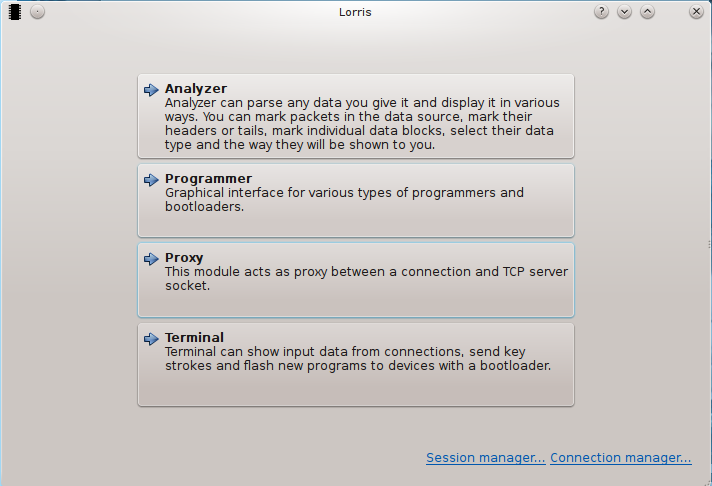
\includegraphics[scale=0.6]{img/new_tab.png}
\caption{Tab creation dialog}
\end{center}
\end{figure}

\begin{figure}[H]
\begin{center}
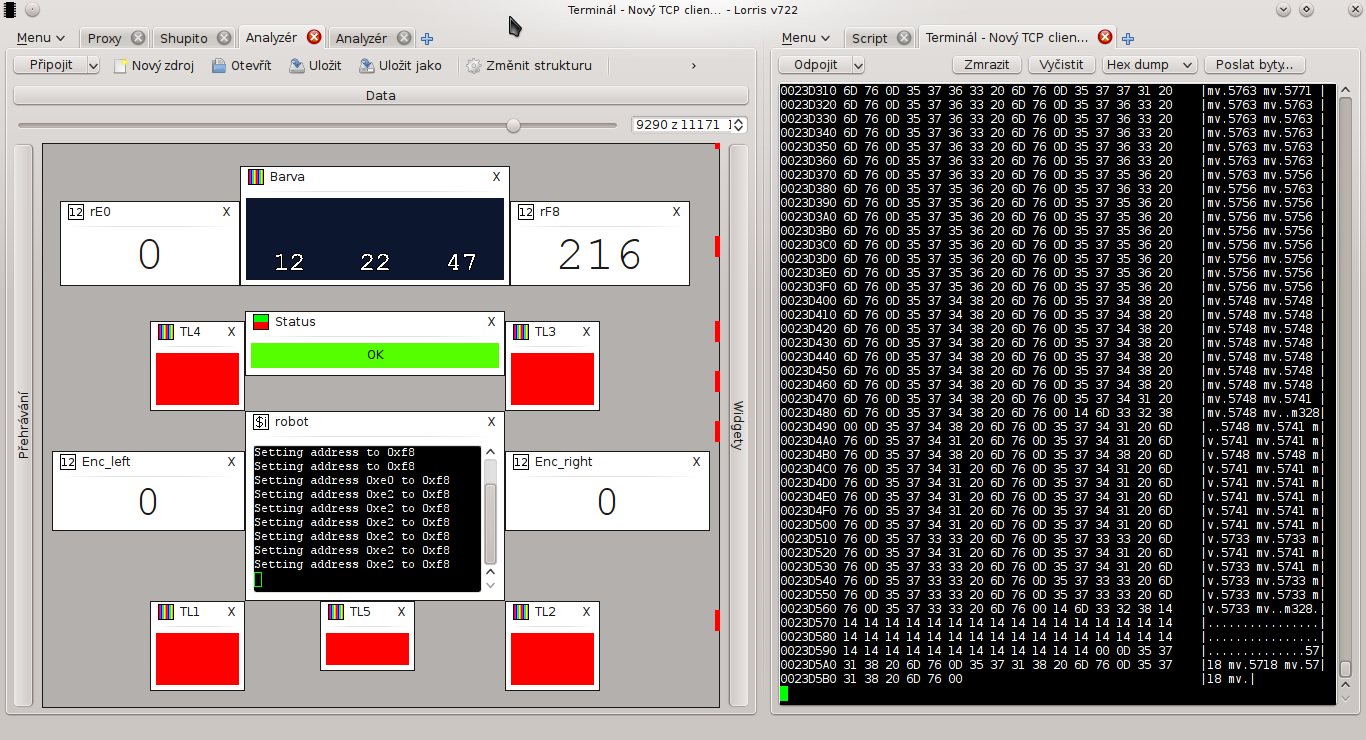
\includegraphics[width=\textwidth]{img/split.png}
\caption{Window divided to multiple parts}
\label{split_img}
\end{center}
\end{figure}

\subsection{Session}
Lorris can save everything user opened (tabs, their layout, connection, data of each tab, ...) as session. User can later load saved session and thus return to his previous work. Lorris automatically saves session before it is closed, so when user starts Lorris again, all his work is in the same state as it was before he left.

\subsection{Automatic updates}
Lorris can update itself under MS Windows. It checks for new version on start, and if there is one available, it shows little notification:
\begin{figure}[H]
\begin{center}

\includegraphics[scale=1]{img/update_notify.png}
\caption{New update notification}
\end{center}
\end{figure}
In case user confirms the update, Lorris closes itself and runs little updater application. Updater shows changelog and downloads new version and installs it.
\begin{figure}[H]
\begin{center}
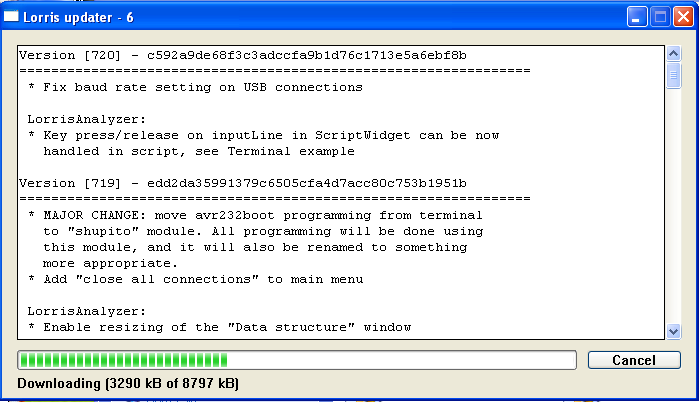
\includegraphics[width=\textwidth]{img/updater.png}
\caption{Ongoing update}
\end{center}
\end{figure}

\newpage
\section{Module: Analyzer}

\begin{figure}[h]
\begin{center}
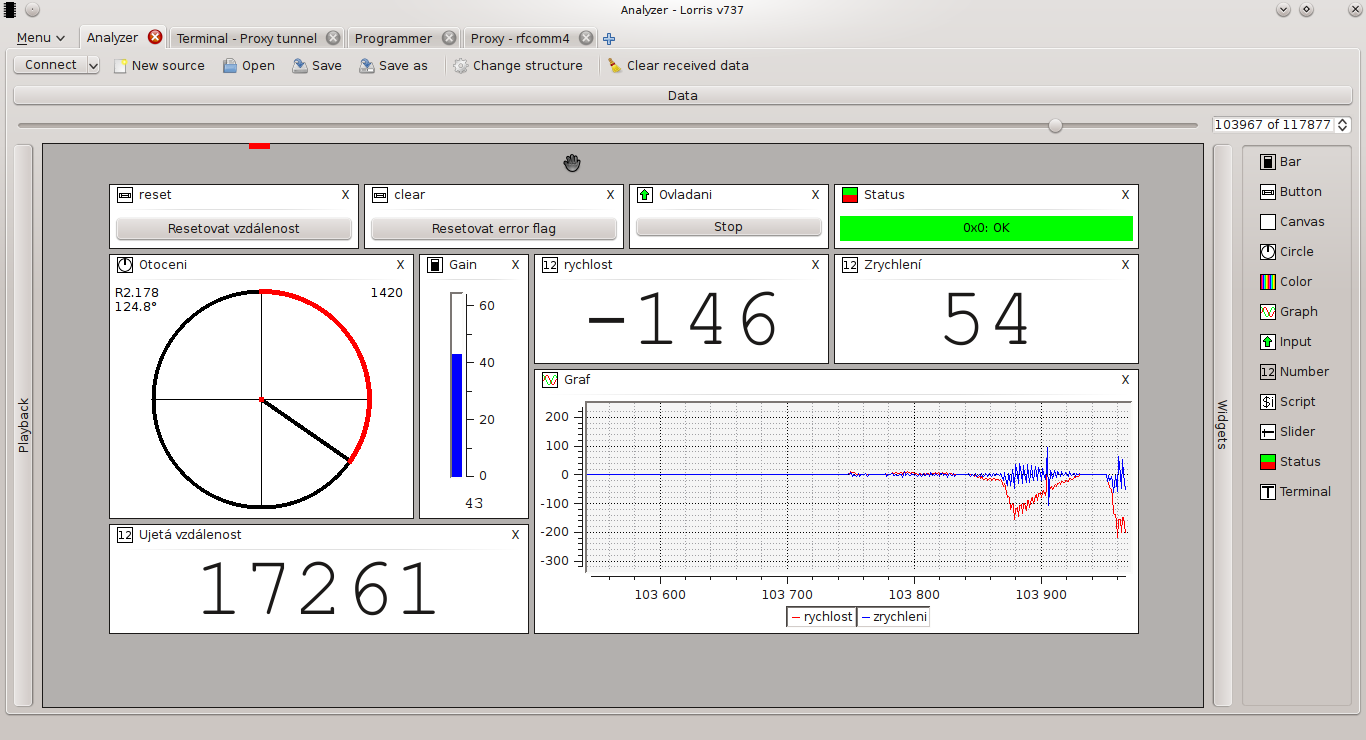
\includegraphics[width=\textwidth]{img/analyzer_all.png}
\caption{Modul analyzer}
\label{Analyzer}
\end{center}
\end{figure}

This module parses incoming data (structured as packets) and displays them in graphical widgets. Application saves processed data into memory -- user can go through received packets using slider and textbox in upper part of the window. All data (received packets, packet structure and widgets positions and settings) can be saved to file. 

Packet structure is configured in dialog window (image \ref{Analyzer_struct}). It is possible to set packet's length, endianness\footnote{\It{Endianness} -- order of bytes in numbers}, packet's header and its content -- static data ("start byte"), dynamic lenght od packet and command and device ID. Packets can be later filtered by command or device ID.

\newpage
\setlength{\voffset}{0mm}
\pagestyle{plain}

Incoming data show up in upper part of the window when packet strcuture is set and user can then "drag" widgets from list in right part of the window to workspace. Data are assigned to widget again using drag\&drop, this time user has to drag first byte of data to widget.

Widget then displays data from that byte (or several bytes if needed). Assigned byte is highlighted when user puts mouse over the widget, so that he can know which data belong to which widget.

Widget settings are available in context menu under right-click. User can set title and other parameters different for each widgets -- these parameters will be described in each widget's section later. Widgets can also be locked, which means the widget can't be closed nor moved or resized.

It is possible to precisely position widgets using grid or by using "aligment lines" (see image \ref{widget_lines}). User can also easily clone widgets by moving them while holding the control key.

Some widgets might profit from following feature: if user grasps widget with mouse as if he wanted to move it and then "shakes it" from right to left, the widget will expand itself to cover all of the visible workspace. When it is moved, it will shrink to it's original size.

\begin{figure}[H]
\begin{center}
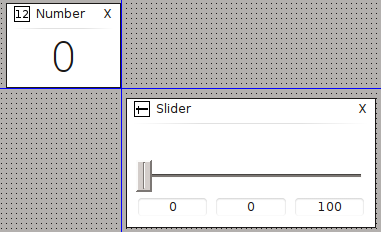
\includegraphics[scale=1]{img/lines.png}
\caption{Widget aligment using grid and lines}
\label{widget_lines}
\end{center}
\end{figure}

\begin{figure}[H]
\begin{center}
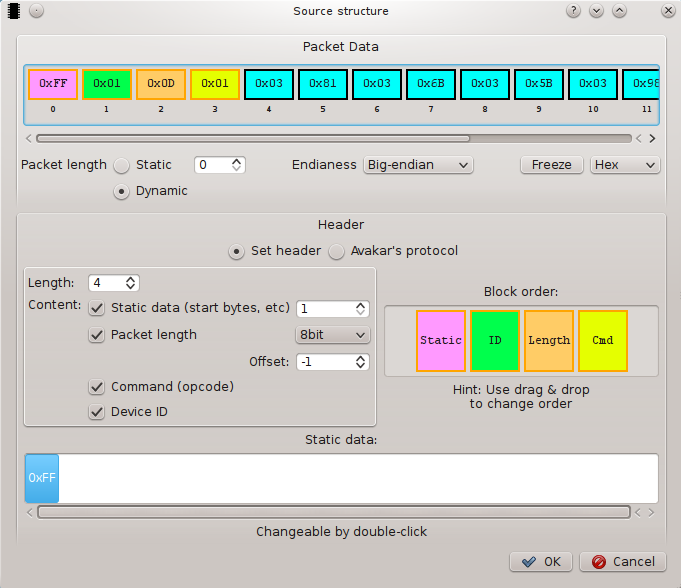
\includegraphics[scale=0.65]{img/analyzer_struct.png}
\caption{Packet structure dialog}
\label{Analyzer_struct}
\end{center}
\end{figure}

\begin{figure}[H]
\begin{center}
\subfloat[List of widgets]{\label{analyzer_widgets}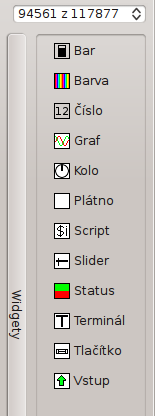
\includegraphics[scale=1]{img/analyzer_widgets_new.png}}
\hfill
\subfloat[Assigning data using drag\&drop]{\label{analyzer_widgets}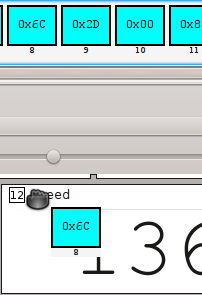
\includegraphics[scale=1]{img/analyzer_drag_data.png}}  
\caption{Widgety}
\label{widgets}
\end{center}
\end{figure}

\subsection{Filters}
Analyzer can filter data using multiple filters at once. Each filter contains conditions, which determine if packet is filtered out or not.
\begin{figure}[H]
\begin{center}
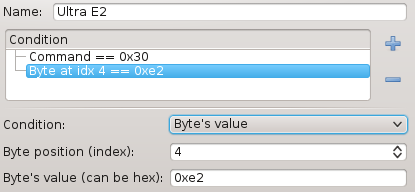
\includegraphics[scale=1]{img/filters.png}
\caption{Filter settings}
\end{center}
\end{figure}
Each condition can check command or device ID from packet's header, value of byte in packet or  it can run simple user script. Thanks to the script, it is possible to write almost any kind of condition.

\begin{listing}[H]
\begin{jscode}
// Return true if passes, false if it
// should be filtered out
function dataPass(data, dev, cmd) {
    return false;
}
\end{jscode}
\caption{Script filter condition}
\end{listing}

% TODO: newpage
\subsection{Widget: number}
\begin{figure}[h]
\begin{center}
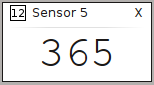
\includegraphics[scale=1]{img/w_num.png}
\caption{Widget: number}
\end{center}
\end{figure}
This widget displays integers (both signed and unsigned, 8 to 64bits) and decimal numbers (single-precision\footnote{Standard floating-point number format used in C and other languages (IEEE 754-2008)}, 32 and 64 bit).
Widget can align the number to max lenght of it's data type and format as follows:
\begin{itemize}
    \item Decimal -- number as base 10
    \item Decimal with exponent -- uses exponent to display big numbers, available only for decimal numbers
    \item Hexadecimal -- number as base 16, available only for unsigned numbers
    \item Binary -- number as base 2, available only for unsigned numbers
\end{itemize}

Another feature is formula to re-calculate widget's value. This is useful for example while showing data from infrared range meters, because their output value must be converted to centimeters using equasion. Formula can look like this:
\begin{center}
\verb|2914/(%n+5)-1|
\end{center}
where \verb|%n| is alias for number which would otherwise be displayed in the widget. This particular formula is for converting distance measured by Sharp GP2Y0A41 infrared range meter to centimeters.

\subsection{Widget: bar}
\begin{figure}[H]
\begin{center}
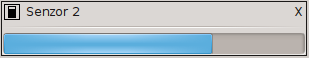
\includegraphics{img/w_bar.png}
\caption{Widget: bar}
\end{center}
\end{figure}
Data in this widget are displayed as bar. User can set data type (same as widget \It{number}), orientation (vertical or horizontal) and range of displayed values. It can also use formula to re-calculate it's value, same as widget \It{number}.

\subsection{Widget: color}
\begin{figure}[H]
\begin{center}
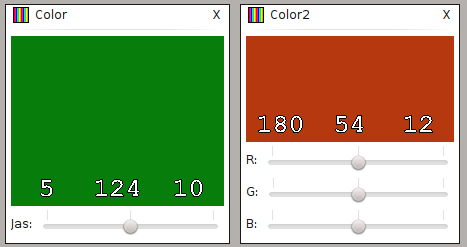
\includegraphics{img/w_col.png}
\caption{Widget: color}
\end{center}
\end{figure}
This widget shows incoming data as colored rectangle. Supported color formats:
\begin{itemize}
    \item {\bf RGB} (8b/channel, 3x uint8)
    \item {\bf RGB} (10b/channel, 3x uint16)
    \item {\bf RGB} (10b/channel, 1x uint32)
    \item {\bf Shades of gray} (8b/channel, 1x uint8)
    \item {\bf Shades of gray} (10b/channel, 1x uint16)
\end{itemize}
Widget supports brightness correction for all colors at once or for each color of RGB space separately.

\subsection{Widget: graph}
\begin{figure}[h]
\begin{center}
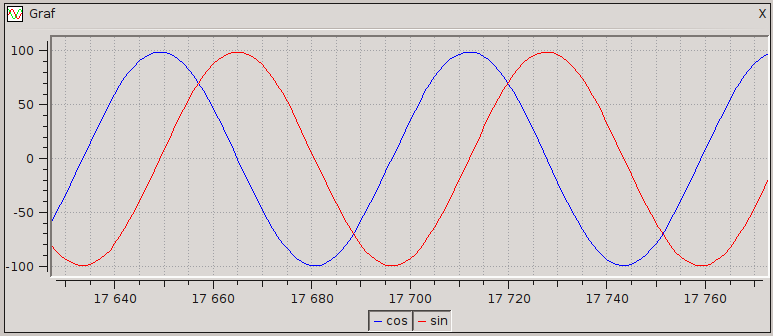
\includegraphics[scale=0.65]{img/w_graph.png}
\caption{Widget: graph}
\end{center}
\end{figure}
This widget shows data in graph -- data order are on  $x$ axis and data values on axis $y$. User can set name, color and data type of each graph curve and automatic scrolling, sample size and scale for graph. Graph also has legend which shows curve's names and colors, and curves can be hidden by clicking at their names in legend. Scale of each axis can be changed by scrolling the mouse wheel while hovering the cursor above axis. If the mouse is above graph area, mousewheel changes scale of both axes at once.
\begin{figure}[h]
\begin{center}
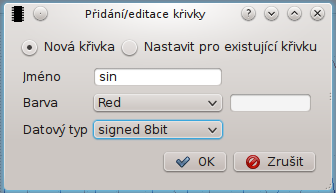
\includegraphics[scale=0.8]{img/w_graph_add.png}
\caption{Curve settings dialog}
\end{center}
\end{figure}

\subsection{Widget: script}
\begin{figure}[h]
\begin{center}
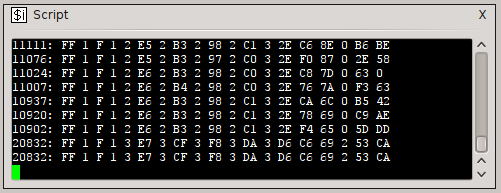
\includegraphics[scale=0.8]{img/w_script.png}
\caption{Widget: script}
\label{script_w}
\end{center}
\end{figure}
This widget uses user-written script to process data. Script can be written in Python or QtScript\cite{qtscript} (language based on ECMAScript\footnote{\It{ECMAScript} -- scripting language accoring to stadard ECMA-262 and ISO/IEC 16262}, same as JavaScript\footnote{\It{JavaScript} -- scripting languge used primarily on web}, so JavaScript and QtScript are very similar).

Script can process incoming data, react to keypresses and send data to device. Basic output can be display in terminal (image \ref{script_w}), but it is also possible to use other widget types to show data (number, bar, ...). Script reference is in \hyperref[script_ref]{attachment A}.

Script editor has buil-in code samples, for example how to set value of existing \It{number} widget, how to send data to device or how to react to keypresses (on image \ref{script_src} are hidden under the lightbulb icon). Editor also has link to automatically generated documentation, which is available on \url{http://technika.junior.cz/docs/Lorris/}.

\begin{figure}[h]
\begin{center}
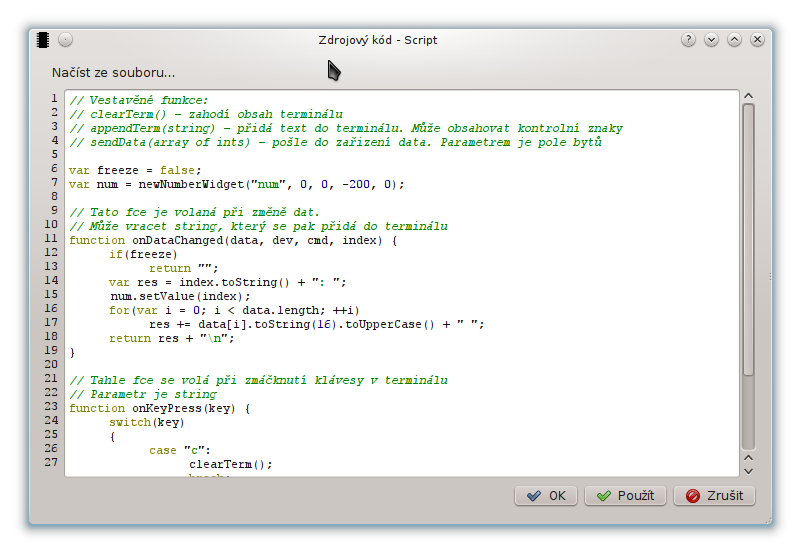
\includegraphics[width=\textwidth]{img/w_script_src.png}
\caption{Script editor}
\label{script_src}
\end{center}
\end{figure}

\subsection{Widget: circle}
\begin{figure}[H]
\begin{center}
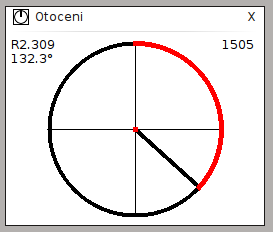
\includegraphics[scale=0.8]{img/w_circle.png}
\caption{Widget: circle}
\end{center}
\end{figure}
Widget circle shows incoming data as angle in circle, which is useful for example when displaying rotation of robot's wheel. Incoming data can be in degrees, radians or just number in certain range (eg. data from 12bit encoder in range from 0 to 4096).

\subsection{Widget: canvas}
\begin{figure}[H]
\begin{center}
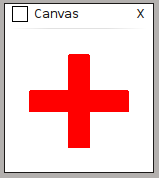
\includegraphics[scale=1]{img/w_canvas.png}
\caption{Widget: canvas}
\end{center}
\end{figure}
Canvas can be only controled from script and is supposed to be used to draw 2D graphics. It can draw lines, rectangles, circles and ellipses. Following code sample will draw red cross in the center of the widget.

\begin{listing}[H]
\begin{jscode}
Canvas.setLineColor("red");
Canvas.setFillColor("red");
// x, y, width, height
Canvas.drawRect(55, 10, 20, 110);
Canvas.drawRect(10, 55, 110, 20);
\end{jscode}
\caption{Drawing to canvas}
\end{listing}

\subsection{Widgets button and slider}
\begin{figure}[H]
\begin{center}
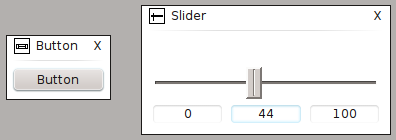
\includegraphics[scale=1]{img/w_btn_slider.png}
\caption{Widgets button and slider}
\end{center}
\end{figure}
These two widgets are used for interaction with script -- callback method in script is invoked in script on button click. In this method user can for example send command to robot. Similarly, callback method is invoked after moving slider, so that user can for example change robot's movement speed. Keyboard shortcut can be assigned to button "click" action and for slider to gain focus, so that user can move it useing arrow keys.
\begin{listing}[H]
\begin{jscode}
function Slider_valueChanged() {
    appendTerm("Slider value: " + Slider.getValue() + "\n");
}

function Button_clicked() {
    appendTerm("Button clicked\n");
}
\end{jscode}
\caption{\It{Slider} and \It{button} callbacks}
\end{listing}

\subsection{Widget: input}
\begin{figure}[H]
\begin{center}
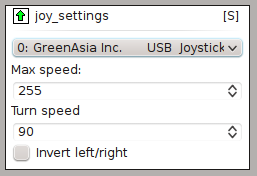
\includegraphics[scale=1]{img/w_input.png}
\caption{Joystick settings in widget \It{input}}
\label{input}
\end{center}
\end{figure}
This widget is also for interaction with script (user \It{input}), but script also defines interface itself -- the widget is empty by default and script has to create UI components, for example button or text field. This widget is a bit more complex, but it can create any of the UI components Qt Framerk contains -- buttons, slider, text fields, combo boxes and so on. Code sample \ref{input_script} creates UI from image \ref{input}.

\begin{listing}[H]
\begin{jscode}
// args: Qt widget name, stretch value
var joyList = joy_settings.newWidget("QComboBox");
var maxSpdLabel = joy_settings.newWidget("QLabel", 1);
var maxSpd = joy_settings.newWidget("QSpinBox");
var turnSpdLabel = joy_settings.newWidget("QLabel", 1);
var turnSpd = joy_settings.newWidget("QSpinBox");
var invert = input.newWidget("QCheckBox");

// set QLabel text
maxSpdLabel.text = "Max speed:";
\end{jscode}
\caption{Adding UI components to widget \It{input}}
\label{input_script}
\end{listing}

\subsection{Widget: status}
\begin{figure}[H]
\begin{center}
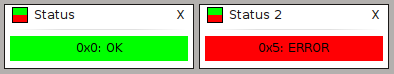
\includegraphics[scale=1]{img/w_status.png}
\caption{Widget status}
\end{center}
\end{figure}
\It{Status} is designed to show state of for example button (pressed/released) or error status from encoder (0 == okay, other values are error codes). User assigns states to incoming values (state consists of text and it's color, see image \ref{status_dlg}) and widget then shows active states. It suports "Unknown value", which is shown when incoming data don't match any defined status.
\begin{figure}[H]
\begin{center}
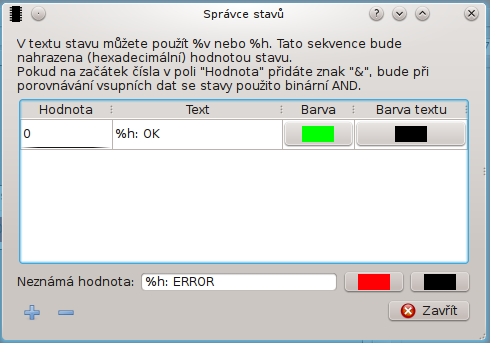
\includegraphics[scale=1]{img/w_status_dlg.png}
\caption{State definitions dialog}
\label{status_dlg}
\end{center}
\end{figure} 

\subsection{Widget: terminal}
\begin{figure}[H]
\begin{center}
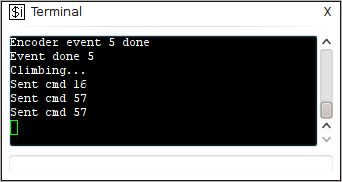
\includegraphics[scale=0.70]{img/w_terminal.png}
\caption{Widget terminál}
\end{center}
\end{figure}
This widget exists only for convenience of the user, it is widget \It{script} with preset code which works exactly as terminal (sending keypresses, showing incoming data). User can edit this predefined script, just like it was regular widget \It{script}.

\newpage
\setlength{\voffset}{0mm} % posune text/obrázek na této stránce, kam patøí
\pagestyle{plain}
\section{Module: Proxy between serial port and TCP socket}
\begin{figure}[H]
\begin{center}
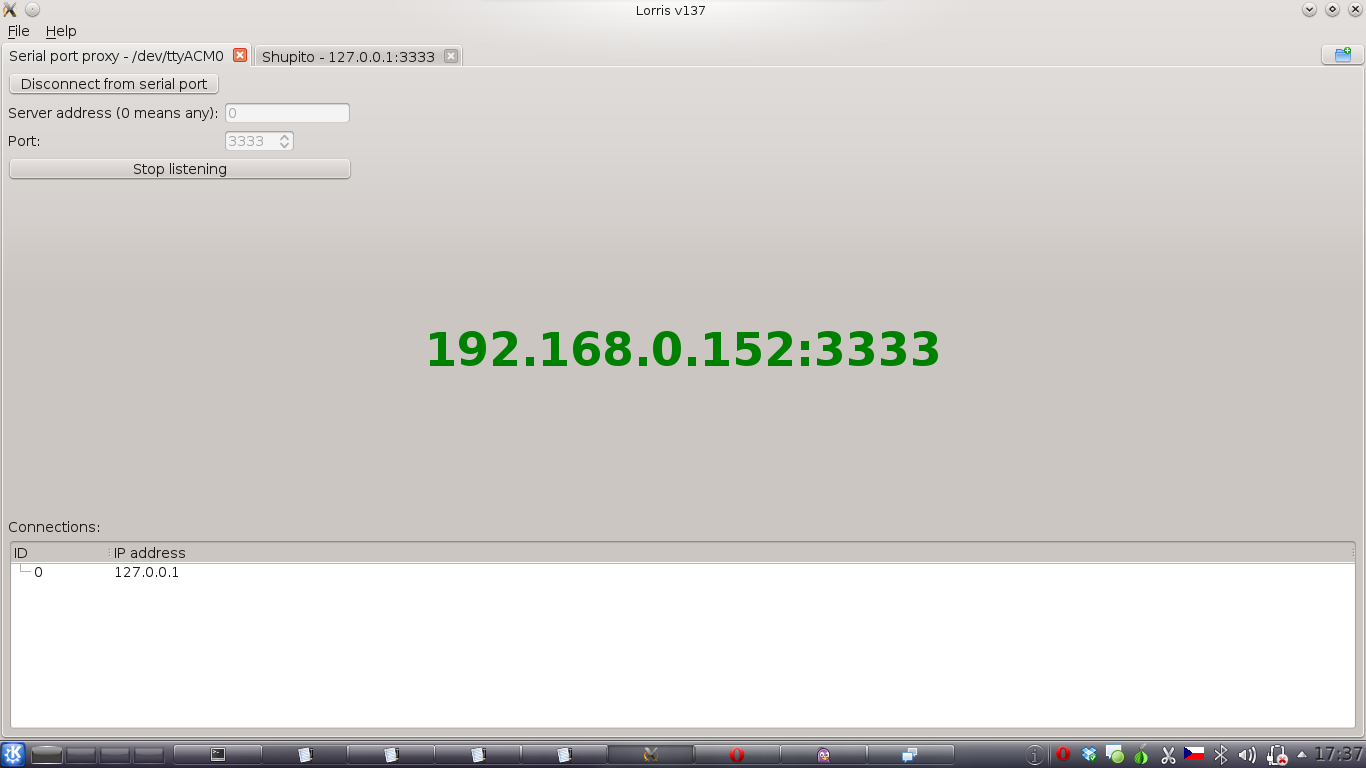
\includegraphics[width=\textwidth]{img/proxy.png}
\caption{Proxy between serial port and TCP socket}
\label{Shupito}
\end{center}
\end{figure}
Simple proxy which transfers data between serial port and TCP socket. It creates server to which user can connect from Lorris or other program on different computer. Data are transfered between serial port and connected clients.

\subsection{Proxy tunnel}
This module also adds new virtual connection - "proxy tunnel". If another Lorris module uses this connection, it can send and receive data from all clients connected to proxy. This can be used to for example generate data in analyzer and then send them to multiple TCP clients.

\newpage
\setlength{\voffset}{0mm} % posune text/obrázek na této stránce, kam patøí
\pagestyle{plain}

\section{Module: programmer}
\begin{figure}[H]
\begin{center}
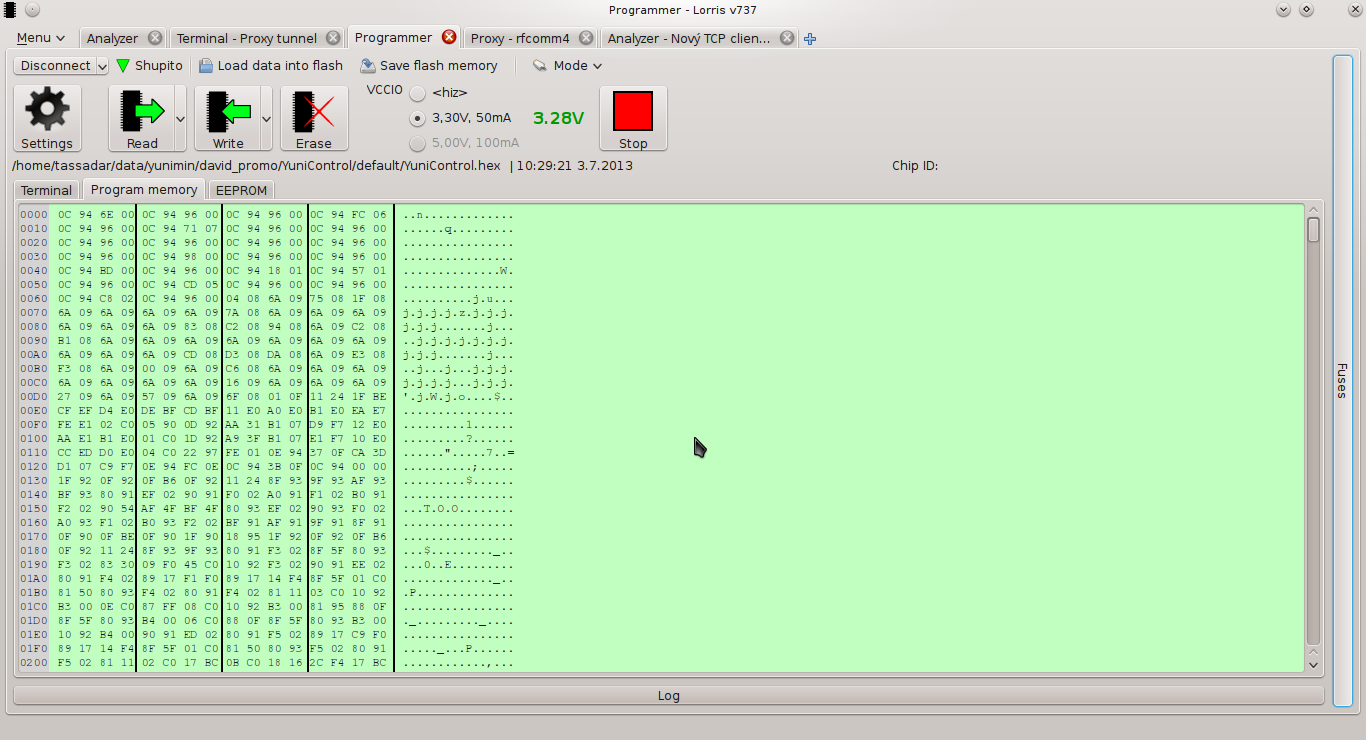
\includegraphics[width=\textwidth]{img/programmer.png}
\caption{Module programmer}
\label{prog_full}
\end{center}
\end{figure}

%TODO: rozšířit
This module acts as graphical interface for several types of programmers and bootloaders. The interface has two modes -- full (image \ref{prog_full}) and minimal (image \ref{prog_mini}. Full interface contains all buttons and settings for programming all memories of the chip, minimal interface contains only button which flashes main memory and button to stop chip. Minimal interface is convenient when using the split feature as demonstrated in image \ref{prog_mini}, because it uses only a small amount of space.

\begin{figure}[H]
\begin{center}
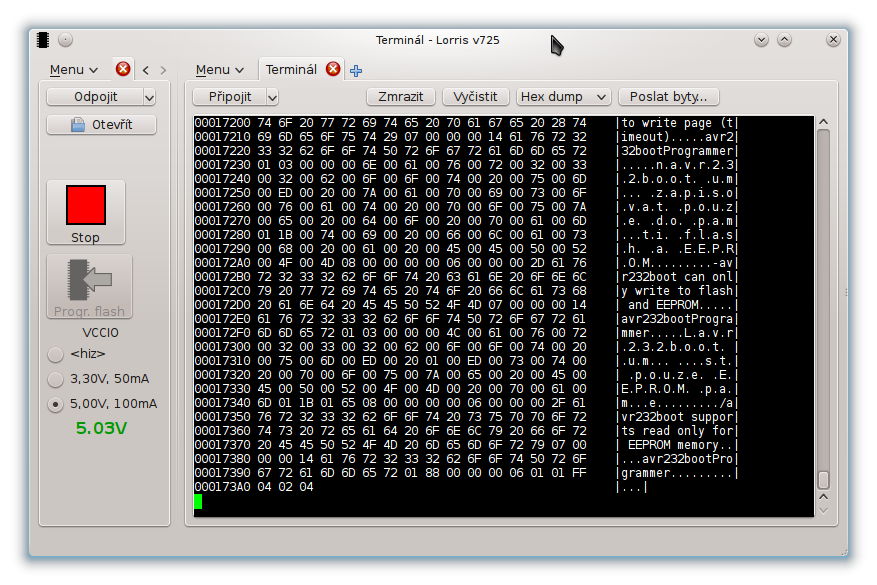
\includegraphics[width=\textwidth]{img/programmer_mini.png}
\caption{Minimal interface of module \It{programmer} (left) along with \It{terminal}}
\label{prog_mini}
\end{center}
\end{figure}

\subsection{Shupito programmer}
Shupito is microchip programmer created by Martin Vejnár. It can program microcontrollers using ISP\footnote{\It{In-system programming} -- interface which can programm chips directly on their PCB}, PDI\footnote{\It{Program and Debug Interface} -- interface by company Atmel with features similar to ISP} a JTAG\footnote{\It{Joint Test Action Group} -- interface standard IEEE 1149.1 which can be used to program and debug chips} interfaces.

Module programmer in Lorris is official interface for Shupito programmer. Most of Shupito communication is written by Martin Vejnár.

\subsubsection{RS232 tunnel}
\label{tunel}
Shupito can create tunnel\footnote{Direct connection between programmed chip and computer via programmer} for RS232 interface from programmed chip to computer. Lorris can use this feature -- active tunnel creates new virtual connection and other modules can connect to it.

\subsection{Bootloader avr232boot}
Author of this bootloader is also Martin Vejnár. Avr232boot supports only Atmel ATmega chips and it is inspired by reference bootloader code for these chips, but it is designed to be as small as possible. It originally could only program flash memory of the chip (the one where program is stored) and I added support for programming and reading of EEPROM\footnote{Flash memory which keeps data even without electricity. It is used to store for example program settings.} memory.

Lorris can use this bootloader to program flash memory and read and program EEPROM.

\subsection{Bootloader AVROSP}
\It{AVR Open Source Programmer} is protocol used by several bootloaders by Atmel for chips ATmega and ATxmega. Lorris can use this protocol to program and read both flash and EEPROM memory of the chip.

\newpage
\section{Module: terminal}
\begin{figure}[H]
\begin{center}
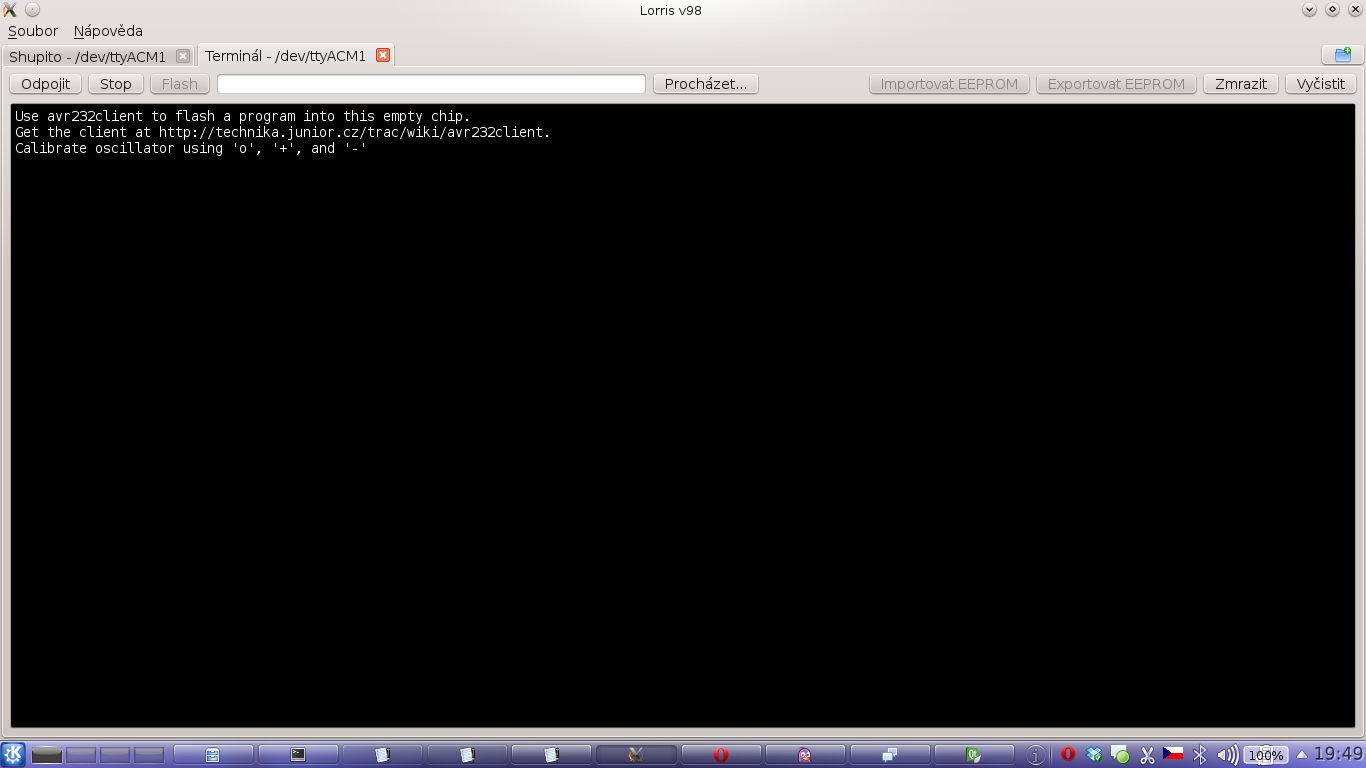
\includegraphics[width=\textwidth]{img/terminal.png}
\caption{Module terminal}
\label{Terminal}
\end{center}
\end{figure}
Fundamental tool for every developer, classic terminal. It shows incoming data in either text mode or as hexadecimal values of each byte and sends keypresses.

User can set terminal's colors, font size, which sequnce of control characters should be send after return key press and behavior of several control characters (for example if character \verb|\n| should create new line or not).

\newpage
\section{Usage examples}
\subsection{Color sensor testing}
{\bf Situation:} I'm builing robot for some competition (Eurobot, RobotChallange, ...) and I want to use color sensor to direct the robot. I also want to test the color sensor, so I've made simple circuit with chip and color sensor. Chip will instruct the sensor to measure the colors and sending color values to computer via RS232 interface.\\
\\
\noindent{\bf Solution:} I use Shupito to program the chip and it's shupito tunnel to read data from RS232 interface. I connect analyzer module to shupito tunnel and then use widget \It{color} to show me color measured by the sensor.

\begin{figure}[h]
\begin{center}
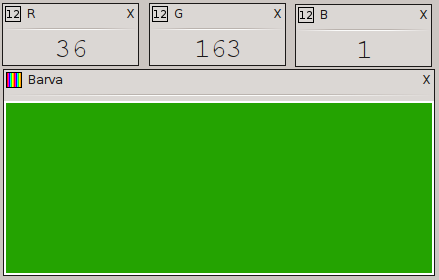
\includegraphics{img/use_color.png}
\caption{Color in analyzer module}
\end{center}
\end{figure}

\newpage
\subsection{Encoder testing}
{\bf Situation:} I need to test the precision of magnetic encoders, but they are sending the angle in several bytes which are not in one sequence, so I can't use terminal.\\
\\
\noindent{\bf Solution:} I don't want to make and program another PCB with chip to process data from encoder, so I connect the encoder to computer and to analyzer module in Lorris. Then I use widget \It{script} to assemble the angle value and to show it in widget \It{number}.

\begin{figure}[H]
\begin{center}
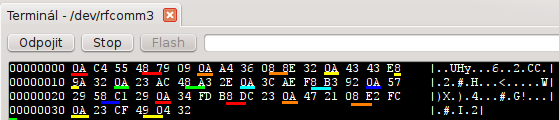
\includegraphics{img/use_enc_term.png}
\caption{Raw encoder data. Highlighted bytes are parts of the angle.}
\end{center}
\end{figure}

\begin{figure}[H]
\begin{center}
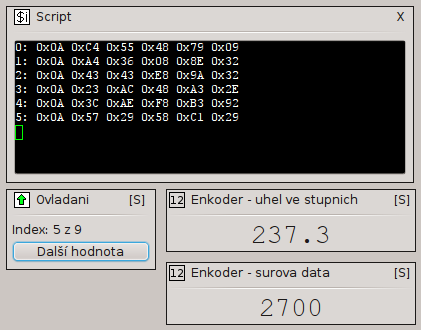
\includegraphics{img/use_enc_analyzer.png}
\caption{Encoder data processed by analyzer}
\end{center}
\end{figure}

\newpage
\subsection{Tuning of PID regulator}
{\bf Situation:} Robot can't go straight because each motor has slightly different speed. I decided to solve this problem using PID regulator. But PID regulator needs several constants to be correctly set. \\
\\
{\bf Solution:} Robot's program is sending current motor speed and PID constants values to computer and also allows changing those constants via RS232 interface. This program is flashed into robot over bluetooth using avr232boot bootloader -- I don't have to use any programmer, which would require cable connection.

I use widgets \It{number} and \It{graph} to show current PID constants and speed of both motors. Then I write simple script which will change PID constants after keypress and starts/stops robot.

I've used this process to tune PID regulator on my 3pi\cite{3pi} robot. I've attened to \It{Line Follower Standard} competition on Robotic Day 2012 in Prague\cite{rob_den} with this robot and I've won second place from total of 22 robots.

\begin{figure}[H]
\begin{center}
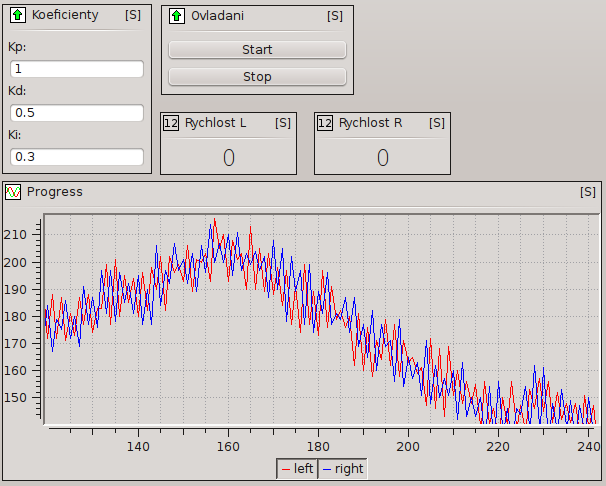
\includegraphics[scale=0.55]{img/use_pid.png}
\caption{PID regulator tuning}
\end{center}
\end{figure}

\newpage
\subsection{Developement of robot for Eurobot 2011 competition}
I've participated in Eurobot\cite{eurobot} contest in 2011. Goal and game mechanics are different each year, in 2011, the goal was to play something like simplified chess game. Game field was colored chessboard and robots were supposed to move "pawns" (yellow discs) to fields of their color and optionally to build towers from said pawns. Winner was the robot with the highest score. Score was calculated by number of built towers and pawns on fields of correct color. In addition to that, robots must not crash into each other, so they must have some means to detect the opponent (eg. ultrasound range meters). You can find complete rules and result list on Eurobot's website\cite{eurobot11}.

Our robot was quite simple, but it had 5 ultrasound range meters, two encoders and 5 buttons nevertheless. These sensors make a lot of data, and terminal is not ideal to show all of them.

\begin{figure}[H]
\begin{center}
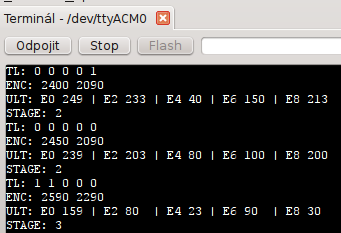
\includegraphics{img/use_david1.png}
\caption{Data from robot in terminal}
\end{center}
\end{figure}

This experience with programming and debugging of robot was one of the main reasons to make this work. If I'd use Lorris to show data from our robot, it would look like this:
\begin{figure}[H]
\begin{center}
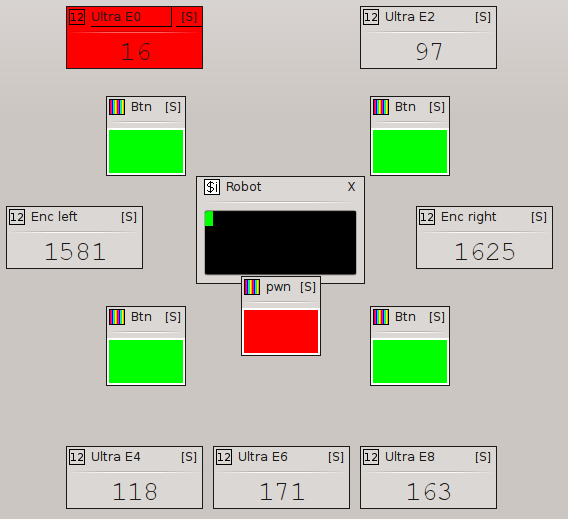
\includegraphics{img/use_david2.png}
\caption{Data simulation in Lorris}
\end{center}
\end{figure}

All the widgets are positioned same as sensors on robot -- 2 ultrasound range meters measure the distance in front and 3 in back; buttons for detecting collisiton with the border are on each corner, button inside the robot checks if robot has pawn inside or not and encoders on both wheels measure the covered distance.

Widget \It{script} named "Robot" in the center represents robot's body. Widgets \It{number} named "Ultra E0..8" display distance measured by the ultrasound meters. Widget "Ultra E0" has value lesser than 25 cm, which means robot has to stop in order not to crash into opponent, so it is colored red.

Widgets \It{color} named "btn" are buttons which detect collision with game field border and "pwn" is button inside robot which is pressed if robot is carrying a pawn. Green means the button is released, red means it is pressed.

And finally, widgets \It{number} named "Enc left" and "Enc right" display distance measured by encoders on right and left wheel.
\begin{figure}[H]
\begin{center}
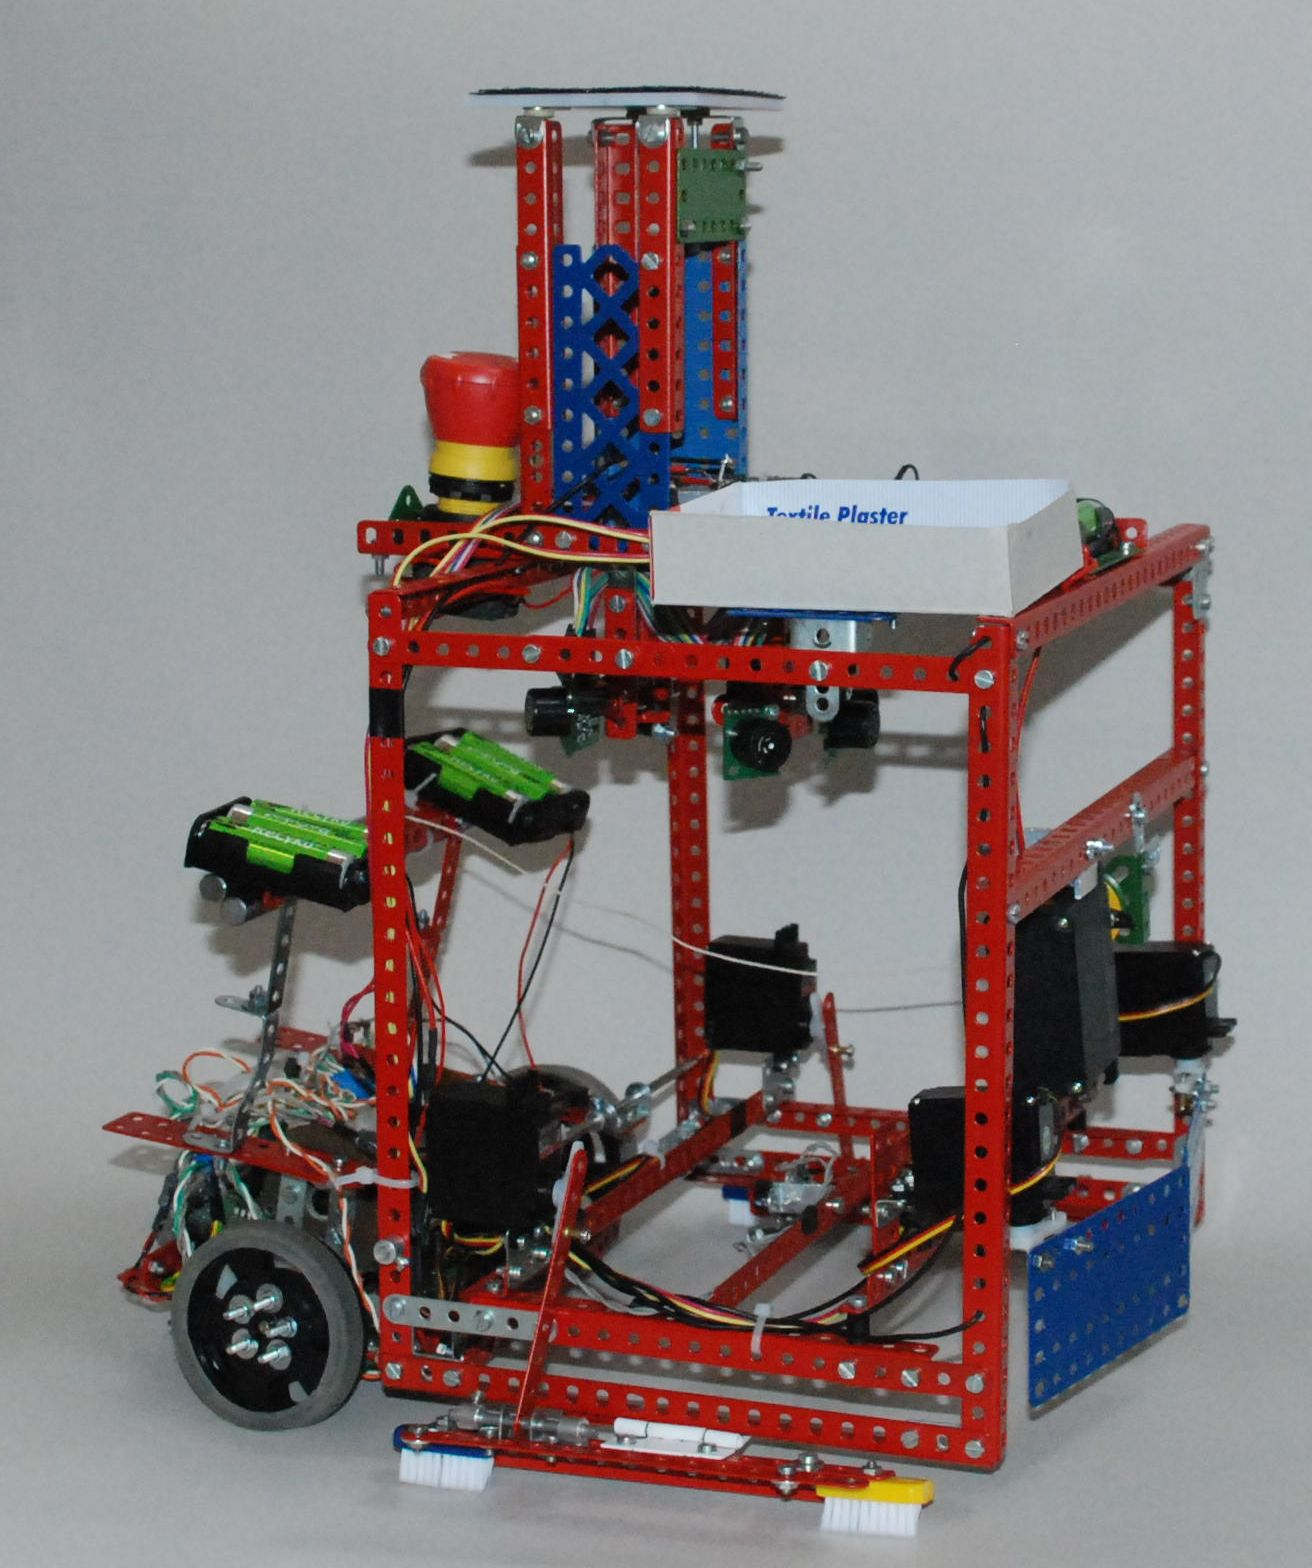
\includegraphics[scale=0.24]{img/use_david_robot.jpg}
\caption{\It{David} -- our robot ended up on the 4th place from total of 11 robots in national Eurobot 2011 competition}
\end{center}
\end{figure}

\section{Joystick support}
Lorris supports joystick in module analyzer to for example control robot. At first, I've used SDL\cite{sdl} library to access joystick, but it was not really suitable for my use -- SDL is video game library, joystick support is only one of many subsystems this library contains. It's architecture also wasn't ideal to use in Lorris.

I haven't found any suitable replacemnt of SDL, so I wrote my own library.

It is called {\bf libenjoy}, it works under Windows and Linux and it is very small and simple. One major advantage over SDL is that it can remember connected joysticks -- if you disconnect joystick and then plug it in again (because you want to reorganize cables on your desktop or because of bad USB connection), it will open the joystick again by itself -- without any user interaction.

Libenjoy is released under GNU LGPLv2.1\cite{lgpl} license.
\begin{itemize}
\item GIT repository: \url{https://github.com/Tasssadar/libenjoy}
\end{itemize}

\newpage
\section{Android application}
\begin{figure}[H]
\begin{center}
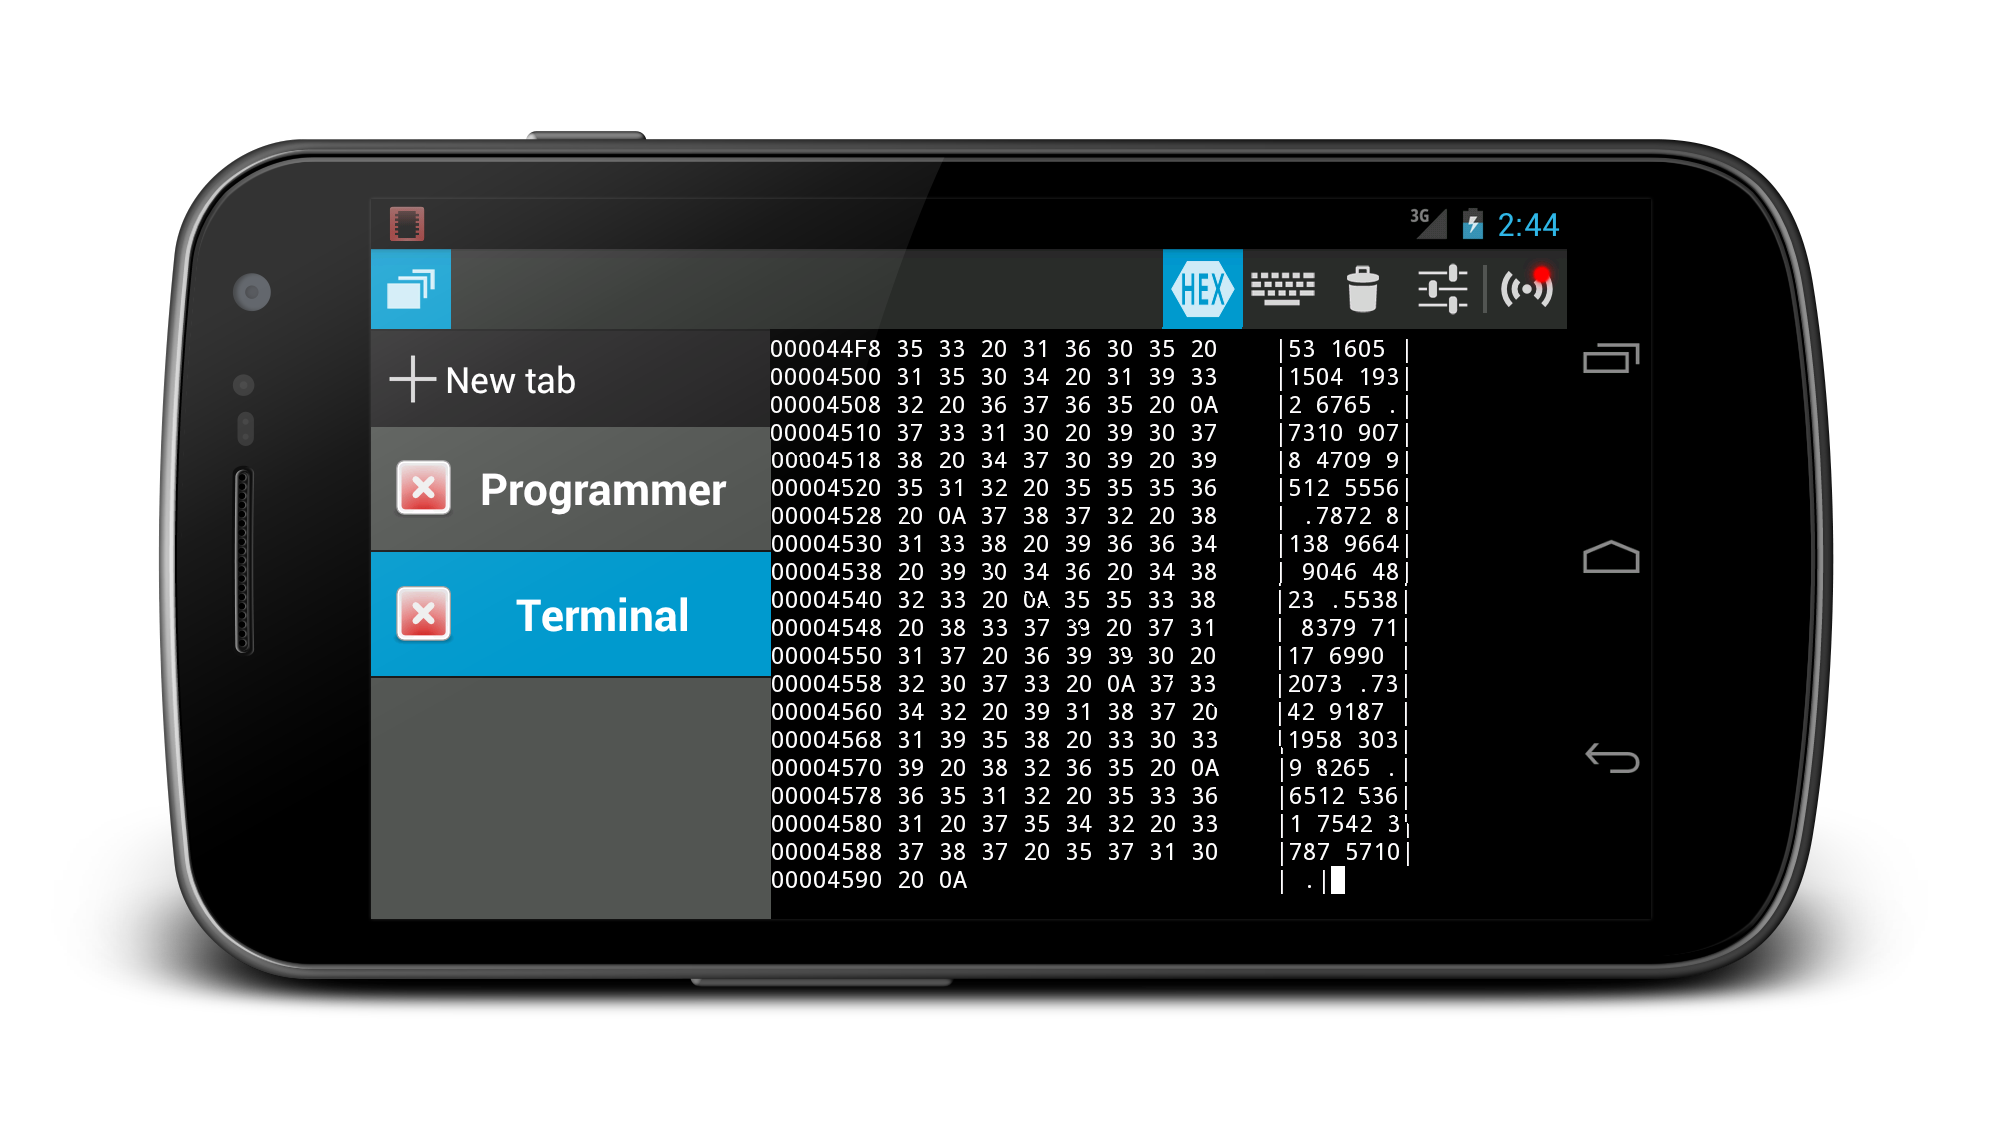
\includegraphics[width=\textwidth]{img/mobile.png}
\caption{Lorris mobile}
\end{center}
\end{figure}

{\bf Lorris mobile} is application for Google Android$^{tm}$ OS and it acts as mobile addition to desktop version of Lorris -- it may not have all the features of desktop versio, but helps when you need to quickly correct or debug something in the field.

App works on all tablets and phones with Android OS version 2.2 and higher, it is optimized also for bigger tablet screens and can be obtained in official distribution channel of Android application -- in Google Play Store\cite{gplay}. You can find it by searching for "Lorris".

Lorris mobile has similiar architecture as desktop Lorris. User has to create session first, so that everything he opens can be saved (image \ref{mobile_session}). After user loads the sessions, he gets to main screen of the application, where he can open modules in tabs, much like in desktop Lorris (image \ref{mobile_tabs}).

\begin{figure}[H]
\begin{center}
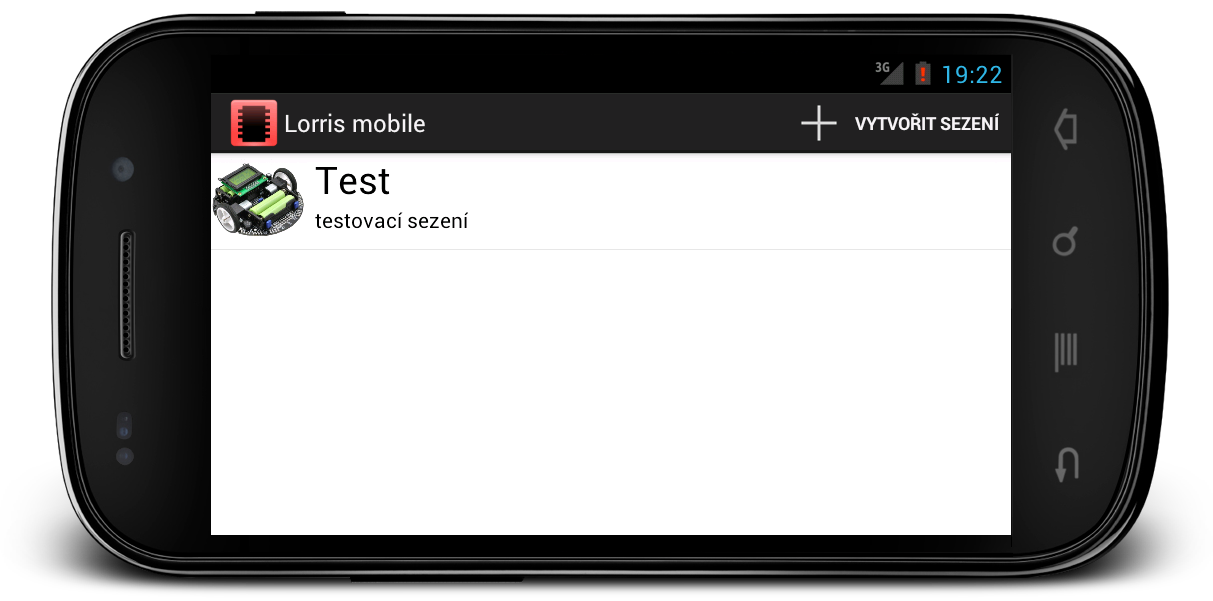
\includegraphics[width=\textwidth]{img/mobile_session.png}
\caption{Lorris mobile -- session selection}
\label{mobile_session}
\end{center}
\end{figure}
\begin{figure}[H]
\begin{center}
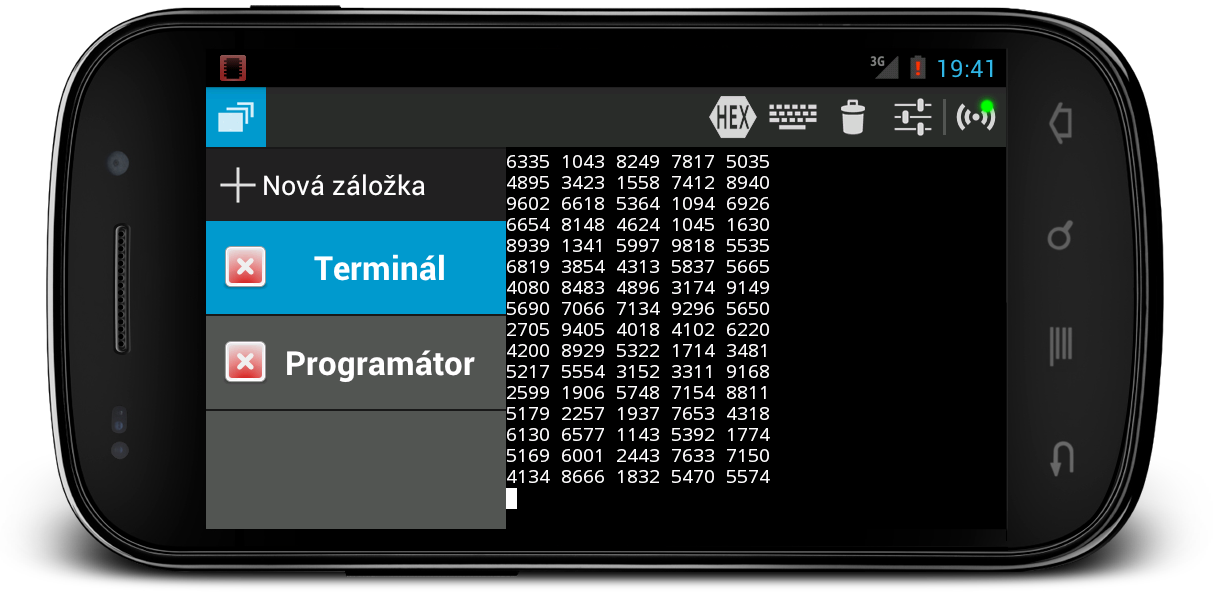
\includegraphics[width=\textwidth]{img/mobile_tabs.png}
\caption{Lorris mobile -- switching tabs}
\label{mobile_tabs}
\end{center}
\end{figure}

\subsection{Programmer}
\begin{figure}[H]
\begin{center}
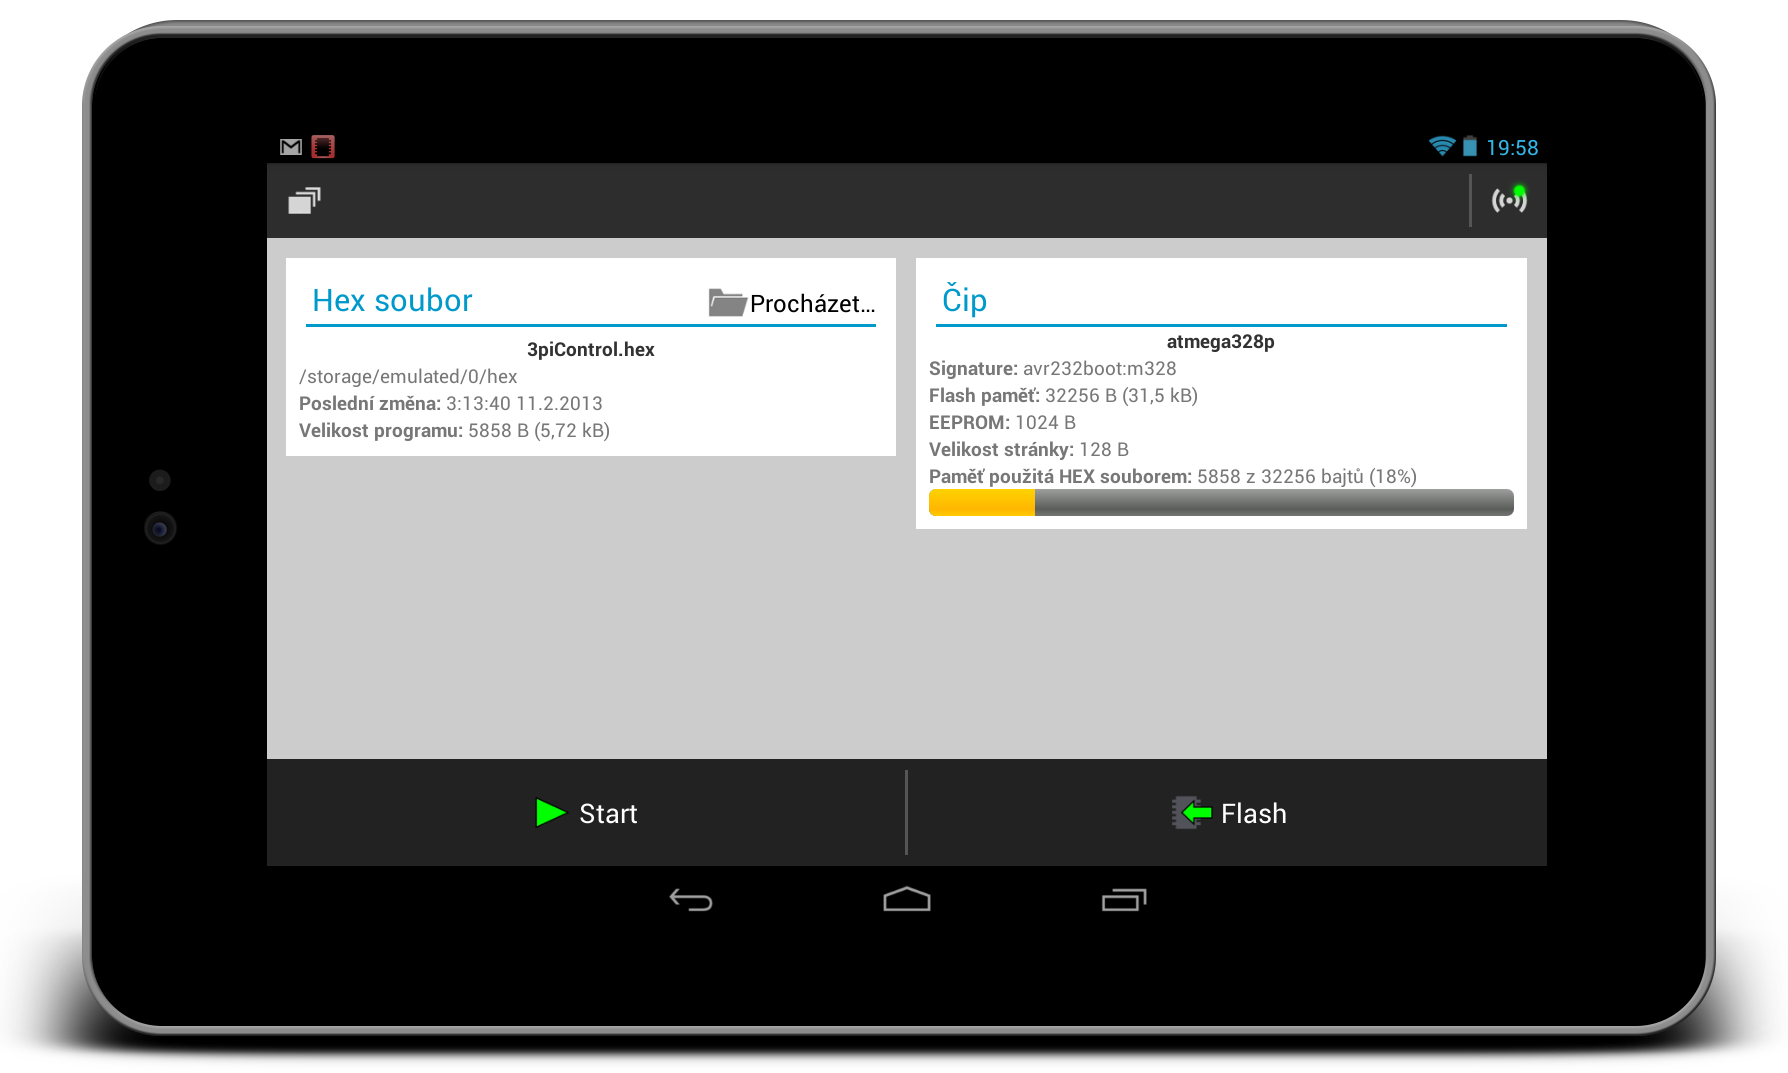
\includegraphics[width=\textwidth]{img/mobile_programmer.png}
\caption{Lorris mobile -- programmer}
\end{center}
\end{figure}
Module programmer can program chips using bootloaders {\bf avr232boot} and {\bf AVROSP} and also using Shupito programmer, if the device has USB host capabilities.

This part of Lorris mobile uses parts of native code from desktop Lorris, which means the code is faster and easier to maintain.

\subsection{Terminal}
\begin{figure}[H]
\begin{center}
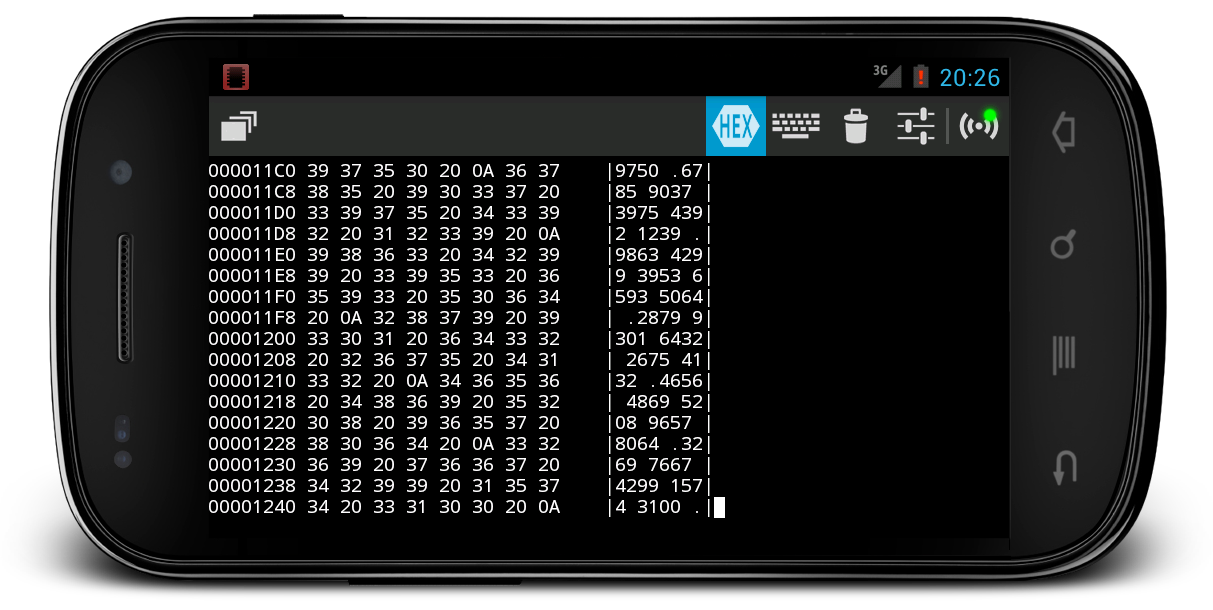
\includegraphics[width=\textwidth]{img/mobile_term.png}
\caption{Lorris mobile -- terminal}
\end{center}
\end{figure}
Classic terminal. Is has most of the features of desktop Lorris -- it displays data (as text or hexadecimal values), sends keypresses and user can set terminal's colors, font size and which control characters are send after return key press.

\newpage
\section*{Conclusion}
\addcontentsline{toc}{section}{Conclusion}
Lorris meets all the requirements which have been set:
\begin{enumerate}[label=\Has\hspace{1.5mm}\arabic{*}.]
    \item Ability to process data from device and cleary show them % 1
    \item Support for many formats of incoming data% 2
    \item Quick and simple to use% 3
    \item Support for other operating systems than MS Windows % 4
    \item Low price% 5
    \item Ability to easily expand program, ideally open-source % 6
    \item No dependencies on other applications (eg. MS Office Excel) % 7
\end{enumerate}
On top of that, the program greatly outdoes original goals -- it also send data to device, program microchips and create proxy between serial port and TCP socket. In comparison to other applications I've found (as described in introduction) Lorris is also the only one which allows user to write his own script to parse data.

Přestože se jedná o zcela nový software, byl již použit při testování barevného senzoru, ladění PID regulátoru pro robota na sledování čáry a je používán pro ovládání programátoru Shupito. Další možnosti použití jsou uvedeny v kapitole 6.

Aplikace je nadále vyvíjena, mohu prakticky donekonečna přídávat buďto další typy widgetů do modulu Analyzér (například kompas, směrový kříž, ...) nebo celé nové moduly (například ovládání robota pomocí joysticku). Program má v současné době (19.4.2012) asi 15 a půl tisíce řádků kódu (bez knihoven třetích stran). Zdrojové kódy a instruktážní video jsou přiloženy na CD. 
\begin{figure}[H]
\begin{center}
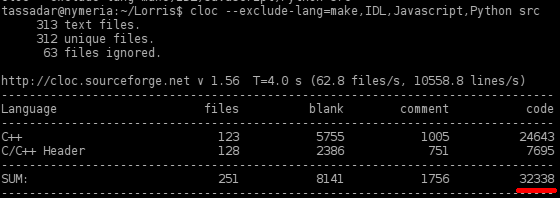
\includegraphics[width=\textwidth]{img/cloc_edit.png}
\caption{Počet řádků spočítaný programem CLOC\cite{cloc}}
\end{center}
\end{figure}

Kromě přidávání dalších vlastností do tohoto programu bych v budoucnu rád vytvořil podobný program (hlavně vlastnosti modulu Analyzér) pro přenosná zařízení (chytrý mobilní telefon či tablet), protože pro tato zařízení žádná taková aplikace v současné době neexistuje a chtěl bych vyzkoušet programování pro tyto platformy (zejména pro Google Android\cite{android}).

%%%%%%%%%%%%%%%%%%%%%%%%%%%%%%%%%%%%%%%%%%%%%%%%%%%%%%%%%%%%%%%%%%%%%%%%%%%
\newpage

%\section*{PŘÍLOHY}
%\addcontentsline{toc}{section}{PŘÍLOHY}

\section*{PŘÍLOHA A:}
\section*{Reference k widgetu \It{script}}
\addcontentsline{toc}{section}{PŘÍLOHA A: Reference k widgetu \It{script}}
\label{script_ref}
Widget \It{script} umožňuje parsování dat pomocí scriptu, který se píše v QtScriptu, který je založený na standardu ECMAScript, na kterém je založený JavaScript. Jazyk je hodně podobný JavaScriptu a většinou můžete použít jeho referenci. Tento text předpokládá alespoň základní znalost JavaScriptu nebo podobného programovacího jazyku.

\begin{itemize}
    \item \url{http://en.wikipedia.org/wiki/ECMAScript}
    \item \url{https://qt-project.org/doc/qt-4.8/scripting.html}
    \item \url{http://www.w3schools.com/jsref/default.asp} -- JS reference
\end{itemize}

\subsubsection*{Online dokumentace}
Ke scriptu je dostupná automaticky generovaná dokumentace, který obsahuje všechny dostupné metody a příklady scriptů:
\begin{itemize}
\item \url{http://technika.junior.cz/docs/Lorris}
\end{itemize}

\newpage
\subsection*{Základní script}
\addcontentsline{toc}{subsection}{Základní script}
Script by může obsahovat následující funkce (ale nemusí, pokud je nepoužívá):
\begin{listing}[H]
\begin{jscode}
function onDataChanged(data, dev, cmd, index) {
    return "";
}

function onKeyPress(key) {
}

function onRawData(data) {
}

function onWidgetAdd(widget, name) {
}

function onWidgetRemove(widget, name) {
}

function onScriptExit() {
}

function onSave() {
}
\end{jscode}
\caption{Základní script}
\label{input_script}
\end{listing}

\noindent{\color{blue}\verb/onDataChanged(data, dev, cmd, index)/} je volána při změně pozice v datech (tj. když přijdou nová data nebo uživatel pohne posuvníkem historie). Může vracet \verb/string/, který se přidá do terminálu.

\begin{itemize}
    \item \verb/data/ -- {\bf pole s Integery} obsahující příchozí data
    \item \verb/dev/ -- {\bf Integer} s ID zařízení (může být definováno v hlavičce packetu -- pokud není, \verb/dev/ se rovná -1)
    \item \verb/cmd/ -- {\bf Integer} s ID příkazu (může být definováno v hlavičce packetu -- pokud není, \verb/cmd/ se rovná -1)
    \item \verb/index/ -- {\bf Integer} s indexem packetu v příchozích datech.
\end{itemize}

\noindent{\color{blue}\verb/onKeyPress(key)/} je volána po stisku klávesy v terminálu.
\begin{itemize}
    \item \verb/key/ -- {\bf String} se stisknutou klávesou
\end{itemize}

\noindent{\color{blue}\verb/onRawData(data)/} je volána kdykoliv příjdou nějáká data.
\begin{itemize}
    \item \verb/data/ -- {\bf pole s bajty} obsahují nenaparsovaná data
\end{itemize}

\noindent{\color{blue}\verb/onWidgetAdd(widget, name)/} \\
{\color{blue}\verb/onWidgetRemove(widget, name)/}

jsou volány při přidání/odebrání widgetu z plochy
\begin{itemize}
    \item \verb/widget/ -- {\bf objekt} widgetu
    \item \verb/name/ -- {\bf String} se jménem widgetu
\end{itemize}

\noindent{\color{blue}\verb/onScriptExit()/} -- tato funkce je volána při ukončení scriptu. Je určena pro ukládání nastavení scriptu.

\noindent{\color{blue}\verb/onSave()/} -- tato funkce je volána těsně prěd uložením dat analyzéru. Je určena pro ukládání nastavení scriptu.

\subsection*{Základní funkce}
\addcontentsline{toc}{subsection}{Základní funkce}
Jsou dostupné základní javascriptové knihovny (\verb/Math/, \verb/Date/, ...) a samotná Lorris poskytuje další rozšiřující funkce. 

\begin{itemize}
    \item {\color{blue}\verb/appendTerm(string)/} -- přidá do terminálu text.\\
        \begin{listing}[H]
        \begin{jscode}
function onKeyPress(key) {
    appendTerm(key); // vypise _key_ do terminalu
}
        \end{jscode}
        \caption{Vypsání stisknutých kláves do terminálu}
        \end{listing}

    \item {\color{blue}\verb/clearTerm()/} -- vyčistí terminál.\\
        \begin{listing}[H]
        \begin{jscode}
function onKeyPress(key) {
    if(key == "c")
        clearTerm(); // vycisti terminal
    else
        appendTerm(key); // vypise _key_ do terminalu
}
        \end{jscode}
        \caption{Vypsání stisknutých kláves do terminálu a jeho vyčištění po stisku klávesy C}
        \end{listing}

    \item {\color{blue}\verb/sendData(pole Integerů)/} \\
         {\color{blue}\verb/sendData(String)/} -- pošle data do zařizení\\
        \begin{listing}[H]
        \begin{jscode}
function onKeyPress(key) {
    sendData(key);
}
        \end{jscode}
        \caption{Poslání ASCII kódu stisknuté klávesy}
        \end{listing}

    \item {\color{blue}\verb/throwException(String)/} -- zobrazí vyskakovací okno s hláškou

    \item {\color{blue}\verb/moveWidget(widget, int x, int y)/} \\
    {\color{blue}\verb/resizeWidget(widget, int sirka, int vyska)/} \\
        Tyto funkce přesunou/změní velikost widgetu. \verb|X| a \verb|Y| jsou absolutní hodnoty na ploše widgetů.

    \item {\color{blue}\verb/newWidget()/} -- tato funkce potřebuje o něco obsáhlejší popis, který je v následující kapitole
\end{itemize}

\subsection*{Vytvoření widgetu}
\addcontentsline{toc}{subsection}{Vytvoření widgetu}

Script může vytvořit všechny ostatní typy widgetů a posílat do nich data. 
{\color{blue}
\begin{verbatim}newWidget(typ, "jméno");
newWidget(typ, "jméno", šířka, výška);
newWidget(typ, "jméno", šířka, výška, Xoffset, Yoffset);
\end{verbatim}
}

\begin{itemize}
    \item \verb|typ| -- {\bf konstanta}, typ widgetu. Používají se tyto konstanty:
    \begin{verbatim}
    WIDGET_NUMBER, WIDGET_BAR, WIDGET_COLOR, WIDGET_GRAPH,
    WIDGET_SCRIPT, WIDGET_INPUT, WIDGET_TERMINAL, WIDGET_BUTTON,
    WIDGET_CIRCLE, WIDGET_SLIDER, WIDGET_CANVAS, WIDGET_STATUS
    \end{verbatim}
    \item \verb/jméno/ -- {\bf String}, jméno widgetu, zobrazí se v titulku
    \item \verb/šířka/ -- {\bf Integer}, šířka widgetu v pixelech. Může být 0, poté se zvolí minimální velikost.
    \item \verb/výška/ -- {\bf Integer}, výška widgetu v pixelech. Může být 0, poté se zvolí minimální velikost.
    \item \verb/Xoffset/ -- {\bf Integer}, vodorovná vzdálenost v pixelech od levého horního rohu mateřského ScriptWidgetu. Může být 0, widget se poté vytvoří v levém horním rohu aktuálně viditelné plochy.
     \item \verb/Yoffset/ -- {\bf Integer}, svislá vzdálenost v pixelech od levého horního rohu mateřského ScriptWidgetu. Může být 0, widget se poté vytvoří v levém horním rohu aktuálně viditelné plochy.
\end{itemize}

\begin{listing}[H]
\begin{jscode}
var cislo = newWidget(WIDGET_NUMBER,
                "rychlost", 200, 100, -250, 0);

function onDataChanged(data, dev, cmd, index) {
    cislo.setValue(data[0]);
    return "";
}
\end{jscode}
\caption{Vytvoření widgetu \It{číslo} a nastavení jeho hodnoty z příchozích dat}
\end{listing}

\subsection*{Dostupné funkce widgetů}
\addcontentsline{toc}{subsection}{Dostupné funkce widgetů}
Objekt widgetu je podtřídou třídy z Qt Frameworku QWidget -- díky tomu může používat jeho vlastnosti a sloty. Popis vlastností najdete v Qt referenci\footnote{\url{http://qt-project.org/doc/qt-4.7/qwidget.html\#propertySection}} v kapitole \uv{Properties} a ve scriptu se používají takto:

\begin{listing}[H]
\begin{jscode}
var cislo = newWidget(WIDGET_NUMBER,
                "rychlost", 200, 100, -250, 0);
cislo.visible = false; // skryti widgetu
\end{jscode}
\caption{Vytvoření widgetu \It{číslo} a nastaveni vlastnosti \uv{visible}}
\end{listing}
Popis slotů je taktéž v Qt referenci, tentokrát pod kapitolou \uv{Public slots}. Používají se jako metody:

\begin{listing}[H]
\begin{jscode}
var cislo = newWidget(WIDGET_NUMBER,
                "rychlost", 200, 100, -250, 0);
cislo.setDisabled(true); // znemozneni interakce s widgetem
\end{jscode}
\caption{Vytvoření widgetu \It{číslo} a použití slotu}
\end{listing}

Kromě těchto zděděných vlastností a funkcí má každý typ widgetu své vlastní.

%\newpage
\subsubsection*{Widget číslo}
\addcontentsline{toc}{subsubsection}{Widget číslo}
\begin{itemize}
    \item {\color{blue}\verb/setValue(Integer nebo double)/} -- Nastaví hodnotu widgetu
    \item {\color{blue}\verb/setFormula(String)/} -- nastaví výraz pro přepočítávání hodnoty
    \item {\color{blue}\verb/setDataType(konstanta)/} -- Nastaví typ vstupu. Konstanty:
        \begin{verbatim}
NUM_UINT8, NUM_UINT16, NUM_UINT32, NUM_UINT64, 
NUM_INT8, NUM_INT16, NUM_INT32, NUM_INT64, 
NUM_FLOAT, NUM_DOUBLE
        \end{verbatim}
\end{itemize}

\begin{listing}[H]
\begin{jscode}
var cislo = newWidget(WIDGET_NUMBER,
                "test cislo", 200, 100, -250, 0);
cislo.setValue(40);
cislo.setFormula("%n-100");
...
cislo.setValue(3.14);
\end{jscode}
\caption{Nastavení hodnoty widgetu \It{číslo}}
\end{listing}

\subsubsection*{Widget sloupcový bar}
\addcontentsline{toc}{subsubsection}{Widget sloupcový bar}
\begin{itemize}
    \item {\color{blue}\verb/setValue(Integer)/} -- Nastaví hodnotu widgetu
    \item {\color{blue}\verb/setRange(Integer min, Integer max)/} -- Nastaví minimální a maximální hodnotu widgetu
    \item {\color{blue}\verb/setRotation(Integer)/} -- Nastaví rotaci sloupce. 0 pro svislou, 1 pro vodorovnou
    \item {\color{blue}\verb/setFormula(String)/} -- nastaví výraz pro přepočítávání hodnoty
    \item {\color{blue}\verb/getMin(), getMax(), getValue()/} -- vrací minimální, maximální a aktualní hodnotu
\end{itemize}

\begin{listing}[H]
\begin{jscode}
var bar = newWidget(WIDGET_BAR, "test bar");
bar.setRange(0, 100); // rozmezi hodnot 0 az 100
bar.setValue(45); // nastaveni hodnoty na 45
bar.setRotation(1); // otoceni na vodorovno
\end{jscode}
\caption{Nastavení hodnot widgetu \It{sloupcový bar}}
\end{listing}

\subsubsection*{Widget barva}
\addcontentsline{toc}{subsubsection}{Widget barva}
\begin{itemize}
    \item {\color{blue}\verb/setValue(Integer r, Integer g, Integer b)/} \\
    {\color{blue}\verb/setValue(String barva)/} \\
    {\color{blue}\verb/setValue(Integer rgb)/} \\
    {\color{blue}\verb/setValueAr(pole integerů)/} \\
        -- Nastaví barvu ve widgetu.
    \item {\color{blue}\verb/setColorType(konstanta)/} -- Nastavý formát vstupu. Konstanty:
        \begin{verbatim}
COLOR_RGB_8, COLOR_RGB_10, COLOR_RGB_10_UINT,
COLOR_GRAY_8, COLOR_GRAY_10
        \end{verbatim}
\end{itemize}

\begin{listing}[H]
\begin{jscode}
var clr = newWidget(WIDGET_COLOR, "test barva");
clr.setValue(255, 255, 0);
clr.setColorType(COLOR_RGB_10);
clr.setValue(543, 1023, 200);
\end{jscode}
\caption{Nastavení hodnot widgetu \It{barva}}
\end{listing}

\subsubsection*{Widget graf}
\addcontentsline{toc}{subsubsection}{Widget graf}
Tento widget se od ostatních poměrně výrazně liší -- je třeba nejdříve vytvořit křivku až té nastavovat hodnoty. Funkce samotného widgetu graf jsou tyto:
\begin{itemize}
    \item {\color{blue}\verb/addCurve(String jméno, String barva)/} -- Vytvoří a vrátí novou křivku. \verb/barva/ může být buďto html název (např. red, blue) nebo HTML hex zápis (např. \#FF0000)
    \item {\color{blue}\verb/removeCurve(String jméno)/} \\
        {\color{blue}\verb/removeAllCurves()/} \\
        Odebrání jedné nebo všech křivek
    \item {\color{blue}\verb/setAxisScale(bool proX, double min, double max)/} -- Nastaví měřítko os. \verb/proX/ je {\bf true} pokud nastavujete měřítko osy $x$
    \item {\color{blue}\verb/updateVisibleArea()/} -- Přesune pohled na nejvyšší hodnotu osy $x$
\end{itemize}

\noindent{\color{blue}\verb/addCurve(String jméno, String barva)/} vrátí křivku, která má tyto funkce:

\begin{itemize}
    \item {\color{blue}\verb/addPoint(Integer index, double hodnota)/} -- Vloží bod křivky. \verb/index/ určuje pořadí bodů (bod s indexem 0 bude vždy před bodem s indexem 50, i když bude vložen až po něm). Pokud bod se stejným indexem už existuje, je jeho hodnota změněna
    \item {\color{blue}\verb/clear()/} -- Smaže všechny body křivky
\end{itemize}

\begin{listing}[H]
\begin{jscode}
var graf = newWidget(WIDGET_GRAPH, "graf", 400, 250, -420, 0);
graf.setAxisScale(false, -105, 105); // meritko osy y
graf.setAxisScale(true, 0, 200); // meritko osy x

// vytvoreni krivky sin
var sin = graf.addCurve("sin", "blue"); 

// pridani bodu do krivky sin
var sinVal = 0;
for(var i = 0; i < 500; ++i) {
    sin.addPoint(i, Math.sin(sinVal)*100);
    sinVal += 0.1;
}
// presunuti na posledni hodnotu krivky
graf.updateVisibleArea(); 
\end{jscode}
\caption{Zobrazení křivky funkce sinus ve widgetu \It{graf}}
\end{listing}

\subsubsection*{Widget vstup}
\addcontentsline{toc}{subsubsection}{Widget vstup}
Tento widget lze vytvořit pouze ze scriptu a umí zobrazit a ovládat většinu Qt widgetů\footnote{\url{http://qt-project.org/doc/qt-4.7/widgets-and-layouts.html}}, například tlačítko (\verb/QPushButton/), zaškrtávací políčko (\verb/QCheckBox/) či textové políčko (\verb/QLineEdit/). Dokumentace k těmto widgetům je v Qt referenci, opět můžete používat vlastnosti (\uv{Properties}) a funkce (\uv{Public slots}).\\
Funkce widgetu \It{vstup}:
\begin{itemize}
    \item {\color{blue}\verb/newWidget(String jméno, Integer roztahování = 0)/} -- Vytvoří a vrátí nový QWidget. \verb/jméno/ musí být jméno třídy widgetu, například QPushButton, QCheckBox nebo QLineEdit. \verb/roztahování/ značí jak moc se bude widget roztahovat oproti ostatním.
    \item {\color{blue}\verb/removeWidget(Objekt widget)/} -- Odstraní widget vrácený voláním \verb|newWidget|.
    \item {\color{blue}\verb/clear()/} -- Odstraní všechny widgety.
    \item {\color{blue}\verb/setHorizontal(bool horizontal)/} -- Nastaví způsob uspořádání widgetů (vedle sebe nebo pod sebou).
\end{itemize}

\begin{listing}[H]
\begin{jscode}
var vstup = newWidget(WIDGET_INPUT,
                "test vstupu", 150, 100, -160, 0);
var label = vstup.newWidget("QLabel", 1);

// zarovnani textu na stred. 
// 0x0080 a 0x0004 jsou konstanty Qt Frameworku 
// Qt::AlignHCenter a Qt::AlignVCenter
label.alignment = 0x0080 | 0x0004;

// nastaveni textu
label.text = "Testovaci popisek";
\end{jscode}
\caption{Widget \It{vstup} -- vytvoření QLabel}
\end{listing}
Widget vytvořený tímto příkladem vypadá takto:

\begin{figure}[H]
\begin{center}
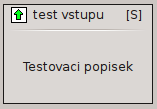
\includegraphics{img/ref_input.png}
\caption{Widget \It{vstup} -- vytvoření QLabel}
\end{center}
\end{figure}

\newpage
QtScript podporuje i využití principu signálů a slotů, díky tomu lze ve scriptu reagovat například na stisknutí tlačítka.

\begin{listing}[H]
\begin{jscode}
var vstup = newWidget(WIDGET_INPUT,
                "test vstupu", 150, 100, -160, 0);

var rychlost = vstup.newWidget("QLineEdit");
rychlost.text = "100";

var btn = vstup.newWidget("QPushButton", 1);
btn.text = "Nastavit";

function posliRychlost() {
    var speed = parseInt(rychlost.text);
    sendData(new Array(speed));
    appendTerm("Rychlost " + speed + "odeslana\n");
}
// Pripojeni signalu "clicked" na slot posliRychlost()
btn.clicked.connect(posliRychlost);
\end{jscode}
\caption{Widget \It{vstup} -- tlačítko}
\end{listing}

\begin{figure}[H]
\begin{center}
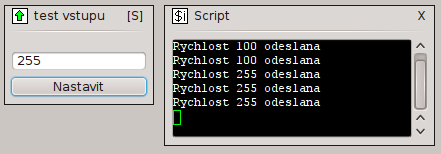
\includegraphics{img/ref_input2.png}
\caption{Widget \It{vstup} -- tlačítko}
\end{center}
\end{figure}

\subsubsection*{Widget kolo}
\addcontentsline{toc}{subsubsection}{Widget kolo}
\begin{itemize}
    \item {\color{blue}\verb/setValue(číslo)/} -- Nastaví zobrazený úhel
    \item {\color{blue}\verb/setClockwise(bool clockwise)/} -- Nastaví jestli se úhel počítá po nebo proti směru hodinových ručiček
    \item {\color{blue}\verb/setAngType(konstanta, min, max/} -- Nastavý vstupní formát. Konstanty:
\verb|ANG_RAD, ANG_DEG, ANG_RANGE|
\end{itemize}

\begin{listing}[H]
\begin{jscode}
var c = newWidget(WIDGET_CIRCLE, "kolo", 200, 200, -210, 0);

c.setAngType(ANG_DEG); // nastaveni vstupu na stupne
c.setValue(270);
\end{jscode}
\caption{Nastavení hodnot widgetu \It{kolo}}
\end{listing}

\subsubsection*{Widget plátno}
\addcontentsline{toc}{subsubsection}{Widget plátno}
\begin{itemize}
    \item {\color{blue}\verb/clear()/} -- Vymaže vše, co je ve widgetu namalované
    \item {\color{blue}\verb/setBackground(String barva)/} -- Nastaví barvu pozadí
    \item {\color{blue}\verb/drawLine(int x1, int y1, int x2, int y2)/} -- Nakreslí čáru.
    \item {\color{blue}\verb/drawLine(int x, int y)/} -- Nakreslí čáru. Začátek je v bodě, kde končí předchozí nakreslená čára (nebo v [0,0] pokud ještě nebyla žádná nakreslená).
    \item {\color{blue}\verb/drawRect(int x, int y, int sirka, int vyska)/} -- Nakreslí obdélník.
    \item {\color{blue}\verb/drawEllipse(int x, int y, int sirka, int vyska)/} -- Nakreslí elipsu
    \item {\color{blue}\verb/drawEllipse(int x, int y, int polomer)/} -- Nakreslí kruh
    \item {\color{blue}\verb/setLineSize(int tloušťka)/} -- Tloušťka čáry, kterou se prvky kreslí.
    \item {\color{blue}\verb/setLineColor(String barva)/} -- Barva čáry, kterou se prvky kreslí.
    \item {\color{blue}\verb/setFillColor(String barva)/} -- Barva výplně obdélníků, elips a kruhů
\end{itemize}

\begin{listing}[H]
\begin{jscode}
var c = newWidget(WIDGET_CANVAS, "Canvas", 140, 170, -150, 0);
c.setLineColor("red");
c.setFillColor("red");

c.drawRect(55, 10, 20, 110);
c.drawRect(10, 55, 110, 20);
\end{jscode}
\caption{Nakreslení kříže ve widgetu \It{plátno}}
\end{listing}

\begin{figure}[H]
\begin{center}
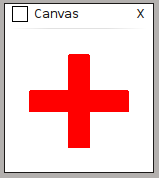
\includegraphics[scale=1]{img/w_canvas.png}
\caption{Nakreslení kříže ve widgetu \It{plátno}}
\end{center}
\end{figure}

\subsubsection*{Widget status}
\addcontentsline{toc}{subsubsection}{Widget status}
\begin{itemize}
    \item {\color{blue}\verb/addStatus(int id, bool bitMaska, String text, String barvaPozadí, String barvaTextu)/} -- Přidá nový status. \verb|bitMask| určuje, zda se má použít přímé porovnání s hodnotou \verb|id| nebo bitový operátor \verb|AND|.
    \item {\color{blue}\verb/removeStatus(int id, bool bitMaska/} -- Odebere status
    \item {\color{blue}\verb/setValue(Integer)/} -- Nastaví vstupní hodnotu
    \item {\color{blue}\verb/getValue()/} -- Vrátí aktuální hodnotu
    \item {\color{blue}\verb/showStatusManager()/} -- Vyvolá dialog pro správu stavů ve widgetu
\end{itemize}

\begin{listing}[H]
\begin{jscode}
var s = newWidget(WIDGET_STATUS, "stav", 0, 0, 200, 0);

s.addStatus(2, false, "Porucha", "orange", "black");
s.setValue(2);
\end{jscode}
\caption{Ovládání widgetu \It{status} ze scriptu}
\end{listing}

\begin{figure}[H]
\begin{center}
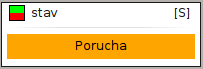
\includegraphics[scale=1]{img/status_script.png}
\caption{Ovládání widgetu \It{status} ze scriptu}
\end{center}
\end{figure}

\subsubsection*{Widget tlačítko}
\addcontentsline{toc}{subsubsection}{Widget tlačítko}
Kromě funkcí, které tento widget má je také možné nastavit metodu která se provede po kliknutí, stačí ve scriptu vytvořit metodu {\color{blue}\verb/JménoWidgetu_clicked()/}.
\begin{itemize}
    \item {\color{blue}\verb/setButtonName(String text)/} -- Nastaví text na tlačítku
    \item {\color{blue}\verb/setShortcut(String zkratka)/} -- Nastaví klávesovou zkratku pro tlačítko
    \item {\color{blue}\verb/setColor(String barva)/} -- Nastaví barvu tlačítka
    \item {\color{blue}\verb/setTextColor(String barva)/} -- Nastaví barvu textu na tlačítku
\end{itemize}

\begin{listing}[H]
\begin{jscode}
var t = newWidget(WIDGET_BUTTON, "tlacitko", 0, 0, 200, 0);

t.setButtonName("Pokus");
t.setShortcut("Ctrl+H");
t.setColor("white");

function tlacitko_clicked() {
    appendTerm("Tlacitko stisknuto!\n");
}
\end{jscode}
\caption{Nastavení widgetu \It{tlačítko} ze scriptu}
\end{listing}

\newpage
\subsubsection*{Widget slider}
\addcontentsline{toc}{subsubsection}{Widget slider}
Kromě funkcí, které tento widget má je také možné nastavit metodu která se provedou při různých změnách stavu slideru. Mají tvar  {\color{blue}\verb/JménoWidgetu_jmenoZmeny()/}, v následujícím příkladě má widget jméno \Uv{Slider}.
\begin{listing}[H]
\begin{jscode}
function Slider_valueChanged() {
    appendTerm("hodnota: " + Slider.getValue() + "\n");
}

function Slider_minimumChanged() {
    appendTerm("nove minimum: " + Slider.getMin() + "\n");
}

function Slider_maximumChanged() {
    appendTerm("nove maximum: " + Slider.getMax() + "\n");
}

function Slider_typeChanged() {
    appendTerm("Typ vstupu zmene na " +
        (Slider.isInteger() ? "Integer" : "Double") + "\n");
}

function Slider_orientationChanged() {
    appendTerm("orientace zmenena na " +
        Slider.getOrientation() + "\n");
}
\end{jscode}
\caption{Funkce, ktere jsou volány při změně stavu widgetu \It{slider}}
\end{listing}
\begin{itemize}
    \item {\color{blue}\verb/setType(bool double)/} -- Nastaví typ hodnot které widget nastavuje (celá nebo desetinná čísla).
    \item {\color{blue}\verb/setMin, setMax, setValue (číslo)/} -- Nastaví minimální, maximální a aktuální hodnotu
    \item {\color{blue}\verb/getMin(), getMax(), getValue()/} -- Vrátí minimální, maximální a aktální hodnotu
\end{itemize}

\begin{listing}[H]
\begin{jscode}
var s = newWidget(WIDGET_SLIDER, "Slider", 0, 0, 300, 0);

s.setType(true); // desetinna cisla
s.setMax(6.28);
s.setValue(3.14);

function Slider_valueChanged() {
    appendTerm("value changed: " + Slider.getValue() + "\n");
}
\end{jscode}
\caption{Ovládání wigetu \It{slider} ze scriptu}
\end{listing}

\newpage
\subsection*{Ukládání dat scriptu}
\addcontentsline{toc}{subsection}{Ukládání dat scriptu}
Na uložení hodnot použitých ve scriptu (například nastavení) je připravena třída \verb|ScriptStorage|. Ve scriptu je dostupná jako objekt \verb|storage| a má tyto funkce:
\begin{itemize}
    \item {\color{blue}\verb/clear()/} -- Vymaže všechna uložená dataPass
    \item {\color{blue}\verb/exists(String klíč)/} -- Vrátí \verb|true| pokud hodnota s tímto klíčem existuje.
    \item {\color{blue}\verb/setXXXX(String klíč, XXX hodnota)/} \\
        {\color{blue}\verb/getXXXX(String klíč, XXX pokudKlíčNeexistuje)/} \\
        {\color{blue}\verb/setYYYYArray(String klíč, PoleYYY hodnota)/} \\
        {\color{blue}\verb/getYYYYArray(String klíč, PoleYYY pokudKlíčNeexistuje)/} \\
            Funkce pro uložení a načtení hodnoty.

        \verb|XXX| typy mohou být \verb|Bool, Uint32, Int32, Float| nebo \verb|String|. Pole \verb|YYYY| může být s prvky typu \verb|UInt32, Int32| nebo \verb|Float|. Druhý parametr u \verb|getXXX| metod je výchozí hodnota, která se vrátí pokud klíč neexistuje.
\end{itemize}

\begin{listing}[H]
\begin{jscode}
var s = newWidget(WIDGET_SLIDER, "Slider", 0, 0, 300, 0);
s.setType(true); // desetinna cisla
s.setMax(6.28);

// Nacte hodnotu, ktera byla pred tim ulozena v metode save()
var ulozene = storage.getFloat("hodnotaPosuvniku", 3.14);
s.setValue(ulozene);

// Nacte pokusne pole cisel ulozene v metode save()
var pokus = storage.getInt32Array("pokusnePole", new Array());
appendTerm("Ulozene pole: " + pokus + "\n");

function onSave() {
    save();
}

function onScriptExit() {
    save();
}

function save() {
    storage.setFloat("hodnotaPosuvniku", Slider.getValue());

    var pokus = new Array(4, 8, 15, 16, 23, 42);
    storage.setInt32Array("pokusnePole", pokus);
}
\end{jscode}
\caption{Ukládání dat scriptu}
\end{listing}

\newpage
\subsection*{Přístup k joysticku}
\addcontentsline{toc}{subsection}{Přístup k joysticku}
Nejříve několik globálních metod pro práci s joysticky:
\begin{itemize}
    \item {\color{blue}\verb/getJoystickNames()/} -- Vráti pole Stringů se jmény přípojených joysticků.
    \item {\color{blue}\verb/getJoystickIds()/} -- Vráti pole Integerů s ID připojených joysticků. Indexy v tomto poli korespondují s polem z funkce \verb|getJoystickNames()|, tj. ID na pozici 0 patří ke jménu na pozici 0.
    \item {\color{blue}\verb/getJoystick(int id)/} -- Otevře joystick s daným ID a vrací object \verb|Joystick| neno NULL pokud nebylo možné joystick otevřit.
    \item {\color{blue}\verb/closeJoystick(Joystick)/} -- Zavře a uvolní objekt joysticku
\end{itemize}
Objekt \verb|joystick| pak má následující metody:
\begin{itemize}
    \item {\color{blue}\verb/getId()/} -- Vrátí ID joysticku
    \item {\color{blue}\verb/getNumAxes()/} \\
          {\color{blue}\verb/getNumButtons()/} -- Vrátí počet os nebo tlačítek
    \item {\color{blue}\verb/getAxisVal(int osa)/} -- Vrátí aktuální hodnotu osy joysticku jako číslo mezi -32768 a 32767. Parametr \verb|osa| je číslo od 0 do \verb|getNumAxes()-1|.
    \item {\color{blue}\verb/getButtonVal(int tlačítko)/} -- Vrátí aktuální hodnotu tlačítka jako číslo 0 (uvolněno) nebo 1 (stisknuto). Parametr \verb|tlačítko| je číslo od 0 do \verb|getNumButtons()-1|.
\end{itemize}
Kromě toho má joystick také dva signály, na které se můžete ve scriptu napojit:
\begin{itemize}
    \item {\color{blue}\verb/axesChanged(Pole integerů)/} -- Volá se když se hodnota některé z os změní. V poli jsou indexy os které se změnily.
    \item {\color{blue}\verb/buttonChanged(int tlačítko, int stav)/} -- Volá se když se zmení stav tlačítka. Parametr \verb|tlačítko| je index tlačítka a \verb|stav| je číslo 0 nebo 1.
\end{itemize}

\begin{listing}[H]
\begin{jscode}
// Pokusi se otevrit prvni dostupny joystick
var ids = getJoystickIds();
var joy = getJoystick(ids[0]);

if(joy) {
    // pripojeni na signaly
    joy.axesChanged.connect(axesChanged);
    joy.buttonChanged.connect(buttonChanged);

    appendTerm("ID joysticku: " + joy.getId() + "\n");
    appendTerm("Pocet os: " + joy.getNumAxes() + "\n");
    appendTerm("Pocet tlacitek: " +
            joy.getNumButtons() + "\n");
}

function axesChanged(axes) {
    for(var i = 0; i < axes.length; ++i) {
        var hodnota = joy.getAxisVal(axes[i]);
        appendTerm("Osa " + axes[i] + ": " + hodnota + "\n");
    }
}

function buttonChanged(id, state) {
    appendTerm("Tlacitko " + id + ", stav: " + state + "\n");
}
\end{jscode}
\caption{Otevření joysticku a čtení jeho hodnot}
\end{listing}
\newpage
\subsection*{Pár věcí, na které je třeba při programování myslet}
\addcontentsline{toc}{subsection}{Pár věcí na které je třeba myslet}
\begin{itemize}
    \item Widgety vytvořené ze scriptu se neukládájí do datového souboru -- po načtení se vytvoří znovu, bez dat.
    \item Stav proměnných ve scritptu se zatím neukládá do souboru.
    \item Po stisknutí \uv{Ok} nebo \uv{Použít} v dialogu nastavení scritpu se script načte znovu -- staré widgety se smažou a vytvoří nové, bez dat.
    \item Jazyk nemá žádné pojistky proti \uv{špatnému} kódu -- pokud ve scritpu bude nekonečná smyčka, Lorris prostě zamrzne
\end{itemize}

\newpage
\section*{PŘÍLOHA B:}
\section*{Knihovny třetích stran}
\addcontentsline{toc}{section}{PŘÍLOHA B: Knihovny třetích stran}
\begin{itemize}
    \item {\bf Qwt}\cite{qwt} je knihovna pro Qt Framework obsahující tzv. widgety pro aplikace technického charakteru -- grafy, sloucové ukazatele, kompasy a podobně. Ve svojí práci zatím z této knihovny používám pouze graf (v modulu analyzéru).
    \item {\bf QExtSerialPort}\cite{qext} poskytuje připojení k sériovému portu a také dokáže vypsat seznam nalezených portů v počítačí.
    \item {\bf QHexEdit2}\cite{qhex} je hex editor použitý v modulu programátoru Shupito na zobrazování obsahu paměti. V této knihovně jsem upravoval několik málo drobností, týkajících se především vzhledu.
\end{itemize}

\section*{PŘÍLOHA C:}
\section*{Licence}
\addcontentsline{toc}{section}{PŘÍLOHA C: Licence}
Lorris je dostupný pod licencí GNU GPLv3\cite{gpl3}, licence použitých programů a knihoven jsou následující:
\begin{itemize}
    \item {\bf Qt Framework} je distribuován pod licencí GNU LGPLv2.1\cite{lgpl}
    \item {\bf Qwt} je distribuováno pod Qwt license\cite{qwtlicense}, která je založená na GNU LGPLv2.1
    \item {\bf QExtSerialPort} je distribuován pod The New BSD License\cite{newbsd}
    \item {\bf QHexEdit2} je distribuován pod licencí GNU LGPLv2.1
    \item {\bf avr232client} je distribuován pod licencí Boost Software License v1.0\cite{boost}
\end{itemize}

Všechny tyto licence umožňují svobodné používání a šíření kódu.

\newpage
 \section*{PŘÍLOHA D:}
 \begin{thebibliography}{99}
\addcontentsline{toc}{section}{PŘÍLOHA D: Reference}
 %% 99 znamená, že maximální délka čísla literatury jsou dva znaky
% seznam samozřejmě změníte podle svého, tohle je pouze ukázka formátování

    \bibitem{serialchart} \It{SerialChart} -- Analyse and chart serial data from RS-232 COM ports \\
    \url{http://code.google.com/p/serialchart/}\\
    (Stav ke dni 6.3.2012)

    \bibitem{winwedge} \It{WinWedge} -- RS232 data collection software \\
    \url{http://www.taltech.com/products/winwedge/}\\
    (Stav ke dni 6.3.2012)

    \bibitem{serialdatalogger} \It{Advanced Serial Data Logger} \\
    \url{http://www.aggsoft.com/serial-data-logger.htm}\\
    (Stav ke dni 6.3.2012)

    \bibitem{stamplot} \It{StampPlot Pro} -- Graphical Data Acquisition and Control \\
    \url{http://www.selmaware.com/stampplot/index.htm}\\
    (Stav ke dni 6.3.2012)

    \bibitem{qtfrm} \It{Qt} -- Cross--platform application and UI framework \\
    \url{http://qt.nokia.com/}\\
    (Stav ke dni 6.3.2012)

    \bibitem{debian} \It{Debian Linux} -- The Universal Operating System \\
    \url{http://www.debian.org/}\\
    (Stav ke dni 6.3.2012)

    \bibitem{github} \It{GitHub} -- Social Coding \\
    \url{https://github.com}\\
    (Stav ke dni 6.3.2012)

    \bibitem{qtscript} \It{Making Applications Scriptable} \\
    \url{http://qt-project.org/doc/qt-4.8/scripting.html}\\
    (Stav ke dni 13.3.2012)

    \bibitem{avr232client} \It{avr232client} \\
    \url{http://technika.junior.cz/trac/wiki/avr232client}\\
    (Stav ke dni 6.3.2012)

    \bibitem{3pi} \It{Pololu 3pi Robot} \\
    \url{http://www.pololu.com/catalog/product/975}\\
    (Stav ke dni 18.4.2012)

    \bibitem{rob_den} \It{Robotický den 2012} \\
    \url{http://www.roboticday.org/cz/}\\
    (Stav ke dni 18.4.2012)

    \bibitem{eurobot} \It{Eurobot} \\
    \url{http://www.eurobot.cz/}\\
    (Stav ke dni 6.3.2012)

    \bibitem{eurobot11} \It{Eurobot 2011} \\
    \url{http://www.eurobot.cz/eurobot2011.php}\\
    (Stav ke dni 6.3.2012)

    \bibitem{sdl} \It{SDL} -- Simple Directmedia Layer \\
    \url{http://www.libsdl.org/}\\
    (Stav ke dni 13.2.2013)

    \bibitem{cloc} \It{CLOC} -- Count Lines of Code \\
    \url{http://cloc.sourceforge.net/}\\
    (Stav ke dni 8.3.2012)

    \bibitem{android} \It{Google Android} -- Operační systém pro chytré telefony\\
    \url{http://www.android.com/}\\
    (Stav ke dni 8.3.2012)

    \bibitem{gplay} \It{Google Play Store} -- Obchod s aplikacemi pro OS Android\\
    \url{http://play.google.com/store}\\
    (Stav ke dni 14.2.2013)

    \bibitem{qwt} \It{Qwt} -- Qt Widgets for Technical Applications \\
    \url{http://qwt.sourceforge.net/}\\
    (Stav ke dni 6.3.2012)

    \bibitem{qext} \It{QExtSerialPort} -- Qt interface class for old fashioned serial ports \\
    \url{http://code.google.com/p/qextserialport/}\\
    (Stav ke dni 6.3.2012)

    \bibitem{qhex} \It{QHexEdit2} -- Binary Editor for Qt \\
    \url{http://code.google.com/p/qhexedit2/}\\
    (Stav ke dni 6.3.2012)

    \bibitem{gpl3} \It{GNU General Public License v3} \\
    \url{http://gplv3.fsf.org/}\\
    (Stav ke dni 6.3.2012)

    \bibitem{lgpl} \It{GNU Lesser General Public License v2.1} \\
    \url{http://www.gnu.org/licenses/lgpl-2.1.html}\\
    (Stav ke dni 6.3.2012)

    \bibitem{qwtlicense} \It{Qwt license} \\
    \url{http://qwt.sourceforge.net/qwtlicense.html}\\
    (Stav ke dni 6.3.2012)

    \bibitem{newbsd} \It{The New BSD License} \\
    \url{http://www.opensource.org/licenses/bsd-license.php}\\
    (Stav ke dni 6.3.2012)

    \bibitem{boost} \It{The Boost Software License} \\
    \url{http://www.boost.org/users/license.html}\\
    (Stav ke dni 6.3.2012)

\end{thebibliography}

\newpage
\section*{PŘÍLOHA E:}
\listoffigures   % seznam obrázkù 
\addcontentsline{toc}{section}{PŘÍLOHA E: Seznam obrázků} % pøidá seznam obrázkù do obsahu 



\end{document}